\documentclass[12pt]{article}
\usepackage[utf8]{inputenc}
\usepackage{tikz}
\usepackage{graphicx}
\usepackage{siunitx} 
\usepackage{subcaption}
\usepackage{float}
\usepackage{amsmath}
\usepackage{multicol}

\title{Lab Investigation: The motion of a Cart rolling down a ramp}
\author{Joshua Liu}
\date{\today}


\begin{document}
\sisetup{ per-mode = symbol } 
\maketitle
\section{Hypothesis}
State the type of motion you think a cart rolling down a ramp will experience as well as justify \textbf{why} you think it will experience this type of motion.

I think the type of motion this cart will experience will be uniform acceleration as the cart is moving down a ramp. I think this will happen as the cart will convert gravitational energy into kinetic energy, meaning there will be constant acceleration.
\section{Procedure}
\begin{enumerate}
    \item Set up an inclined plane as shown in the given Figure. Clamp the timer near the top of the board. Set up a fixed stop at the bottom of the board.
    \item Obtain a length of ticker tape slightly shorter than the incline ramp. Feed the tape through the timer and attach the end of the tape to the back of the cart.
    \item Turn on the timer and allow the cart to roll down the incline ramp. Have your partner stop the cart at the end of the ramp.
    \item Choose a clear dot at the beginning to be the reference point at the time of $0.00 s$. The timer likely makes dots at a frequency of $60 Hz$. The time interval between two points is $\frac{1}{60} s$. For convenience, mark off intervals every six dots along the tape so that each interval represents $0.10 s$ up to $2.0 s$ 20 dots.
    \item Measure the position of the cart with respect to the reference point after $0.10 s$, and record the data in a position-time table.
    \begin{center}
        \begin{tabular}{c|c @{\hspace{5em}} c|c}
            \multicolumn{2}{c}{Trial 1}&\multicolumn{2}{c}{Trial 2}\\
            \hline
            Time&Position&Time&Position\\
            0.0 & 0.000 & 0.0 & 0.000\\
            0.1 & 0.005 & 0.1 & 0.004\\
            0.2 & 0.012 & 0.2 & 0.010\\
            0.3 & 0.024 & 0.3 & 0.019\\
            0.4 & 0.042 & 0.4 & 0.030\\
            0.5 & 0.063 & 0.5 & 0.043\\
            0.6 & 0.089 & 0.6 & 0.059\\
            0.7 & 0.113 & 0.7 & 0.076\\
            0.8 & 0.150 & 0.8 & 0.099\\
            0.9 & 0.187 & 0.9 & 0.116\\
            1.0 & 0.226 & 1.0 & 0.138\\
            1.1 & 0.270 & 1.1 & 0.161\\
            1.2 & 0.318 & 1.2 & 0.184\\
            1.3 & 0.369 & 1.3 & 0.209\\
            1.4 & 0.423 & 1.4 & 0.234\\
            1.5 & 0.481 & 1.5 & 0.260\\
            1.6 & 0.543 & 1.6 & 0.287\\
            1.7 & 0.608 & 1.7 & 0.314\\
            1.8 & 0.676 & 1.8 & 0.343\\
            1.9 & 0.750 & 1.9 & 0.372\\
            2.0 & 0.825 & 2.0 & 0.401\\

        \end{tabular}
    \end{center}
    \item Before you dismantle the ramp, measure the height of textbooks (H) and the length of the ramp (L) to measure the angle of inclination of the ramp.
    \begin{itemize}
        \item Trial 1, 5 Textbooks: $H=0.118m, L=2.27m$
        \item Trial 2, 3 Textbooks: $H=0.071m, L=2.27m$
    \end{itemize}
    \item Use the formula $\theta=sin^{-1}(\frac{H}{L})$ to find the angle of inclination of the ramp.
    \begin{itemize}
        \item Trial 1, $\theta= sin^{-1}(\frac{0.118}{2.27})=2.99^{\circ}$
        \item Trial 2, $\theta= sin^{-1}(\frac{0.071}{2.27})=1.79^{\circ}$
    \end{itemize}
    \item Repeat the previous steps for one more different angle to have a total of two trials.
\end{enumerate}

\section{Analysis}

\subsection{Graphical Method}
\begin{enumerate}
    \item Use the position and time data that you collected in the procedure to plot a position-time graph for the motion of the cart down the ramp for every trial.
    \begin{figure}[H]
        \centering
        \begin{minipage}{0.4\textwidth}
            \centering
            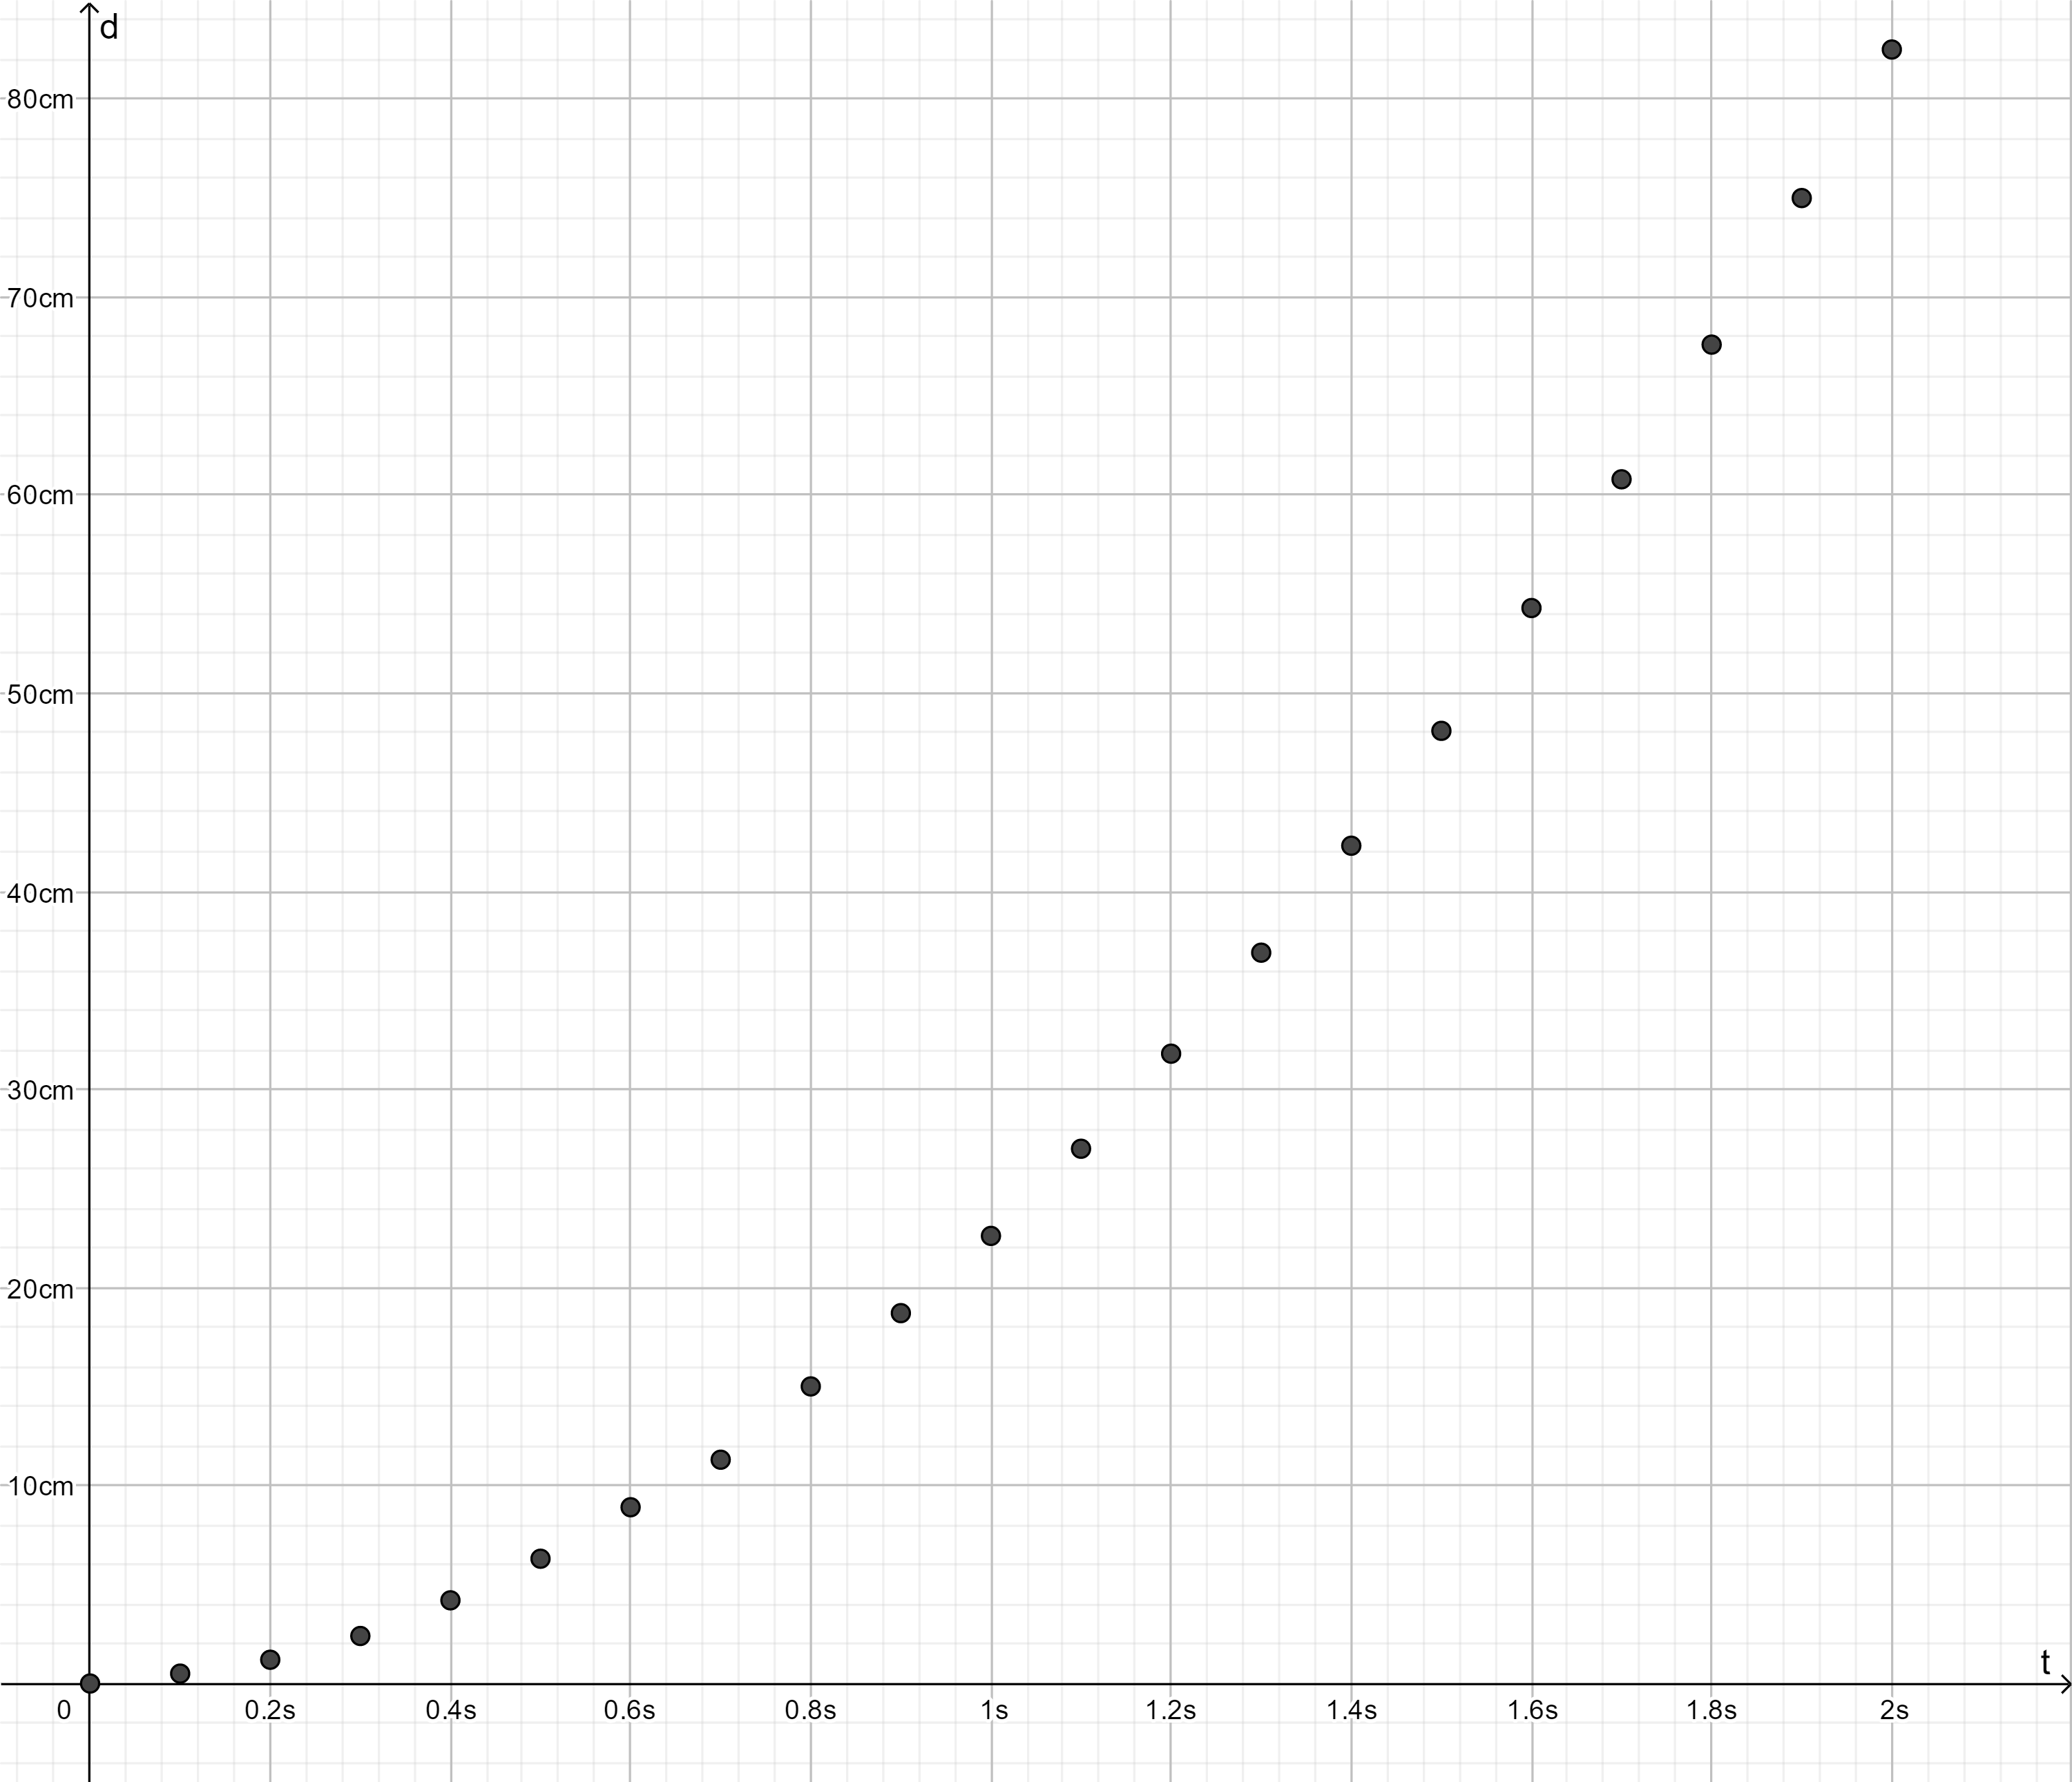
\includegraphics[scale=2]{LabReportImg/5TB.png}
            \captionof*{figure}{Trial one}
        \end{minipage}
        \begin{minipage}{0.4\textwidth}
            \centering
            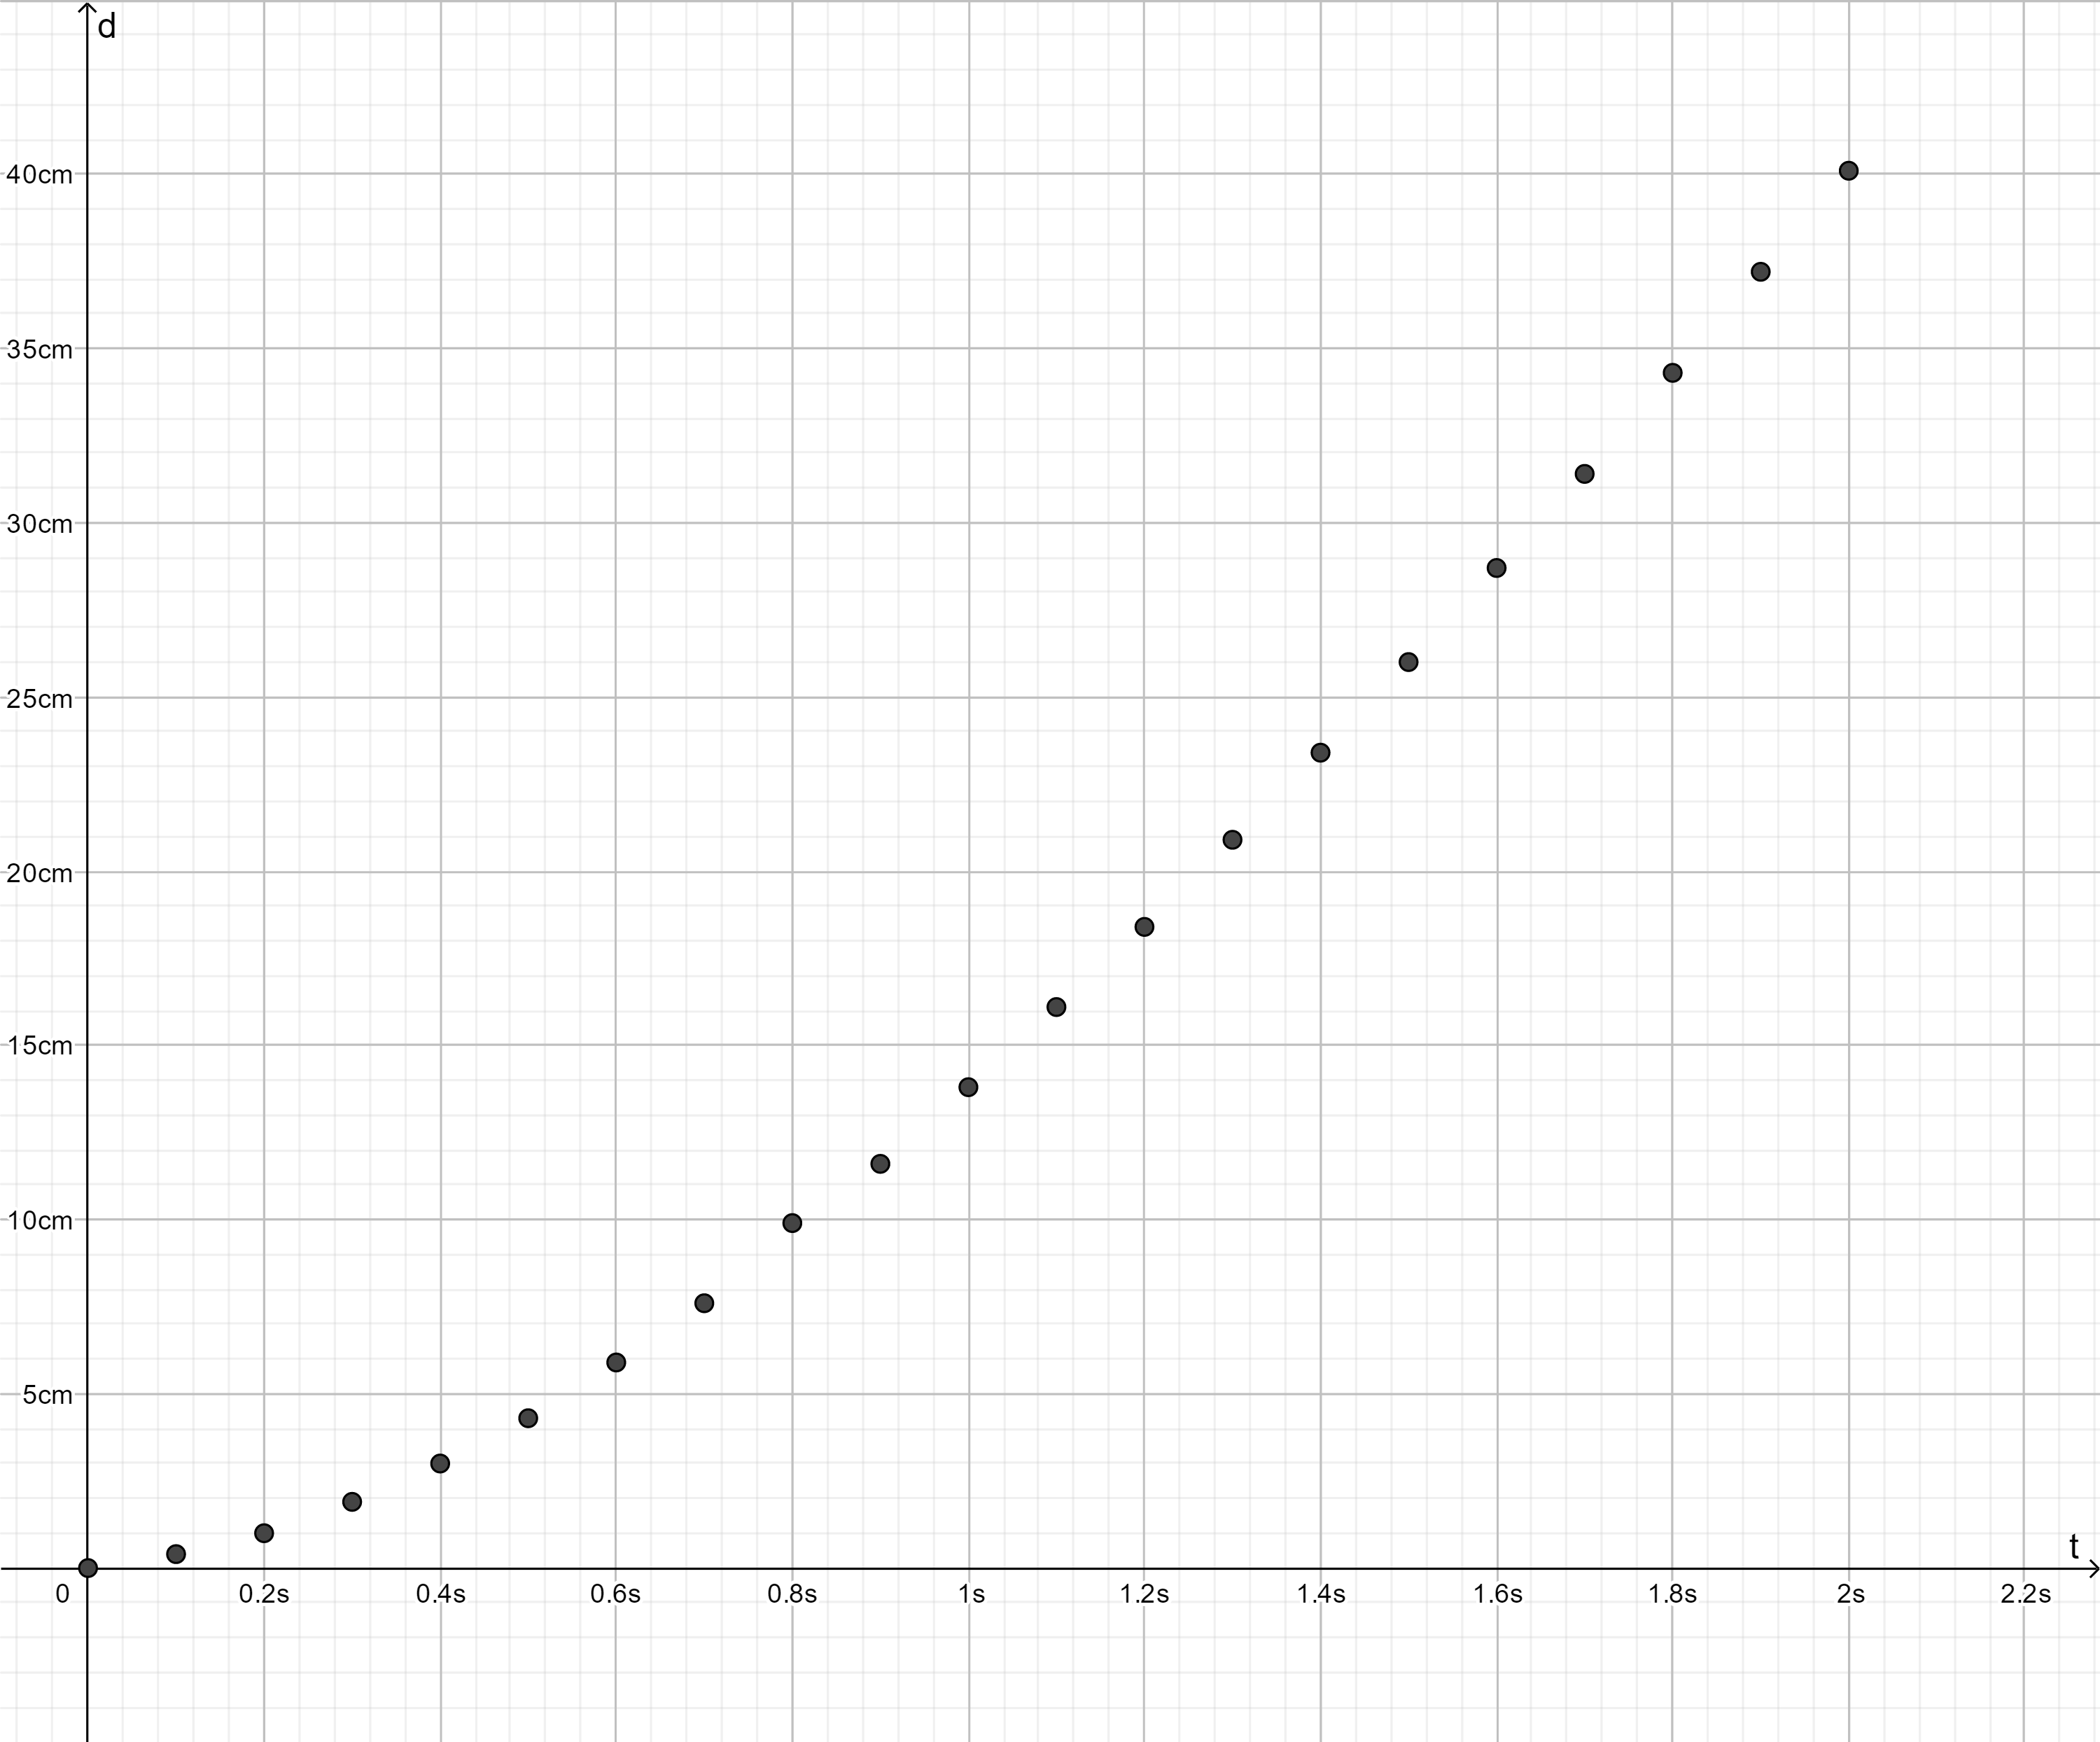
\includegraphics[scale=2]{LabReportImg/3TB.png}
            \captionof*{figure}{Trial two}
        \end{minipage}
    \end{figure}
    \item Draw tangents of the cart every $0.60$ s at three specific times.
    \begin{figure}[H]
        \centering
        \begin{minipage}{0.4\textwidth}
            \centering
            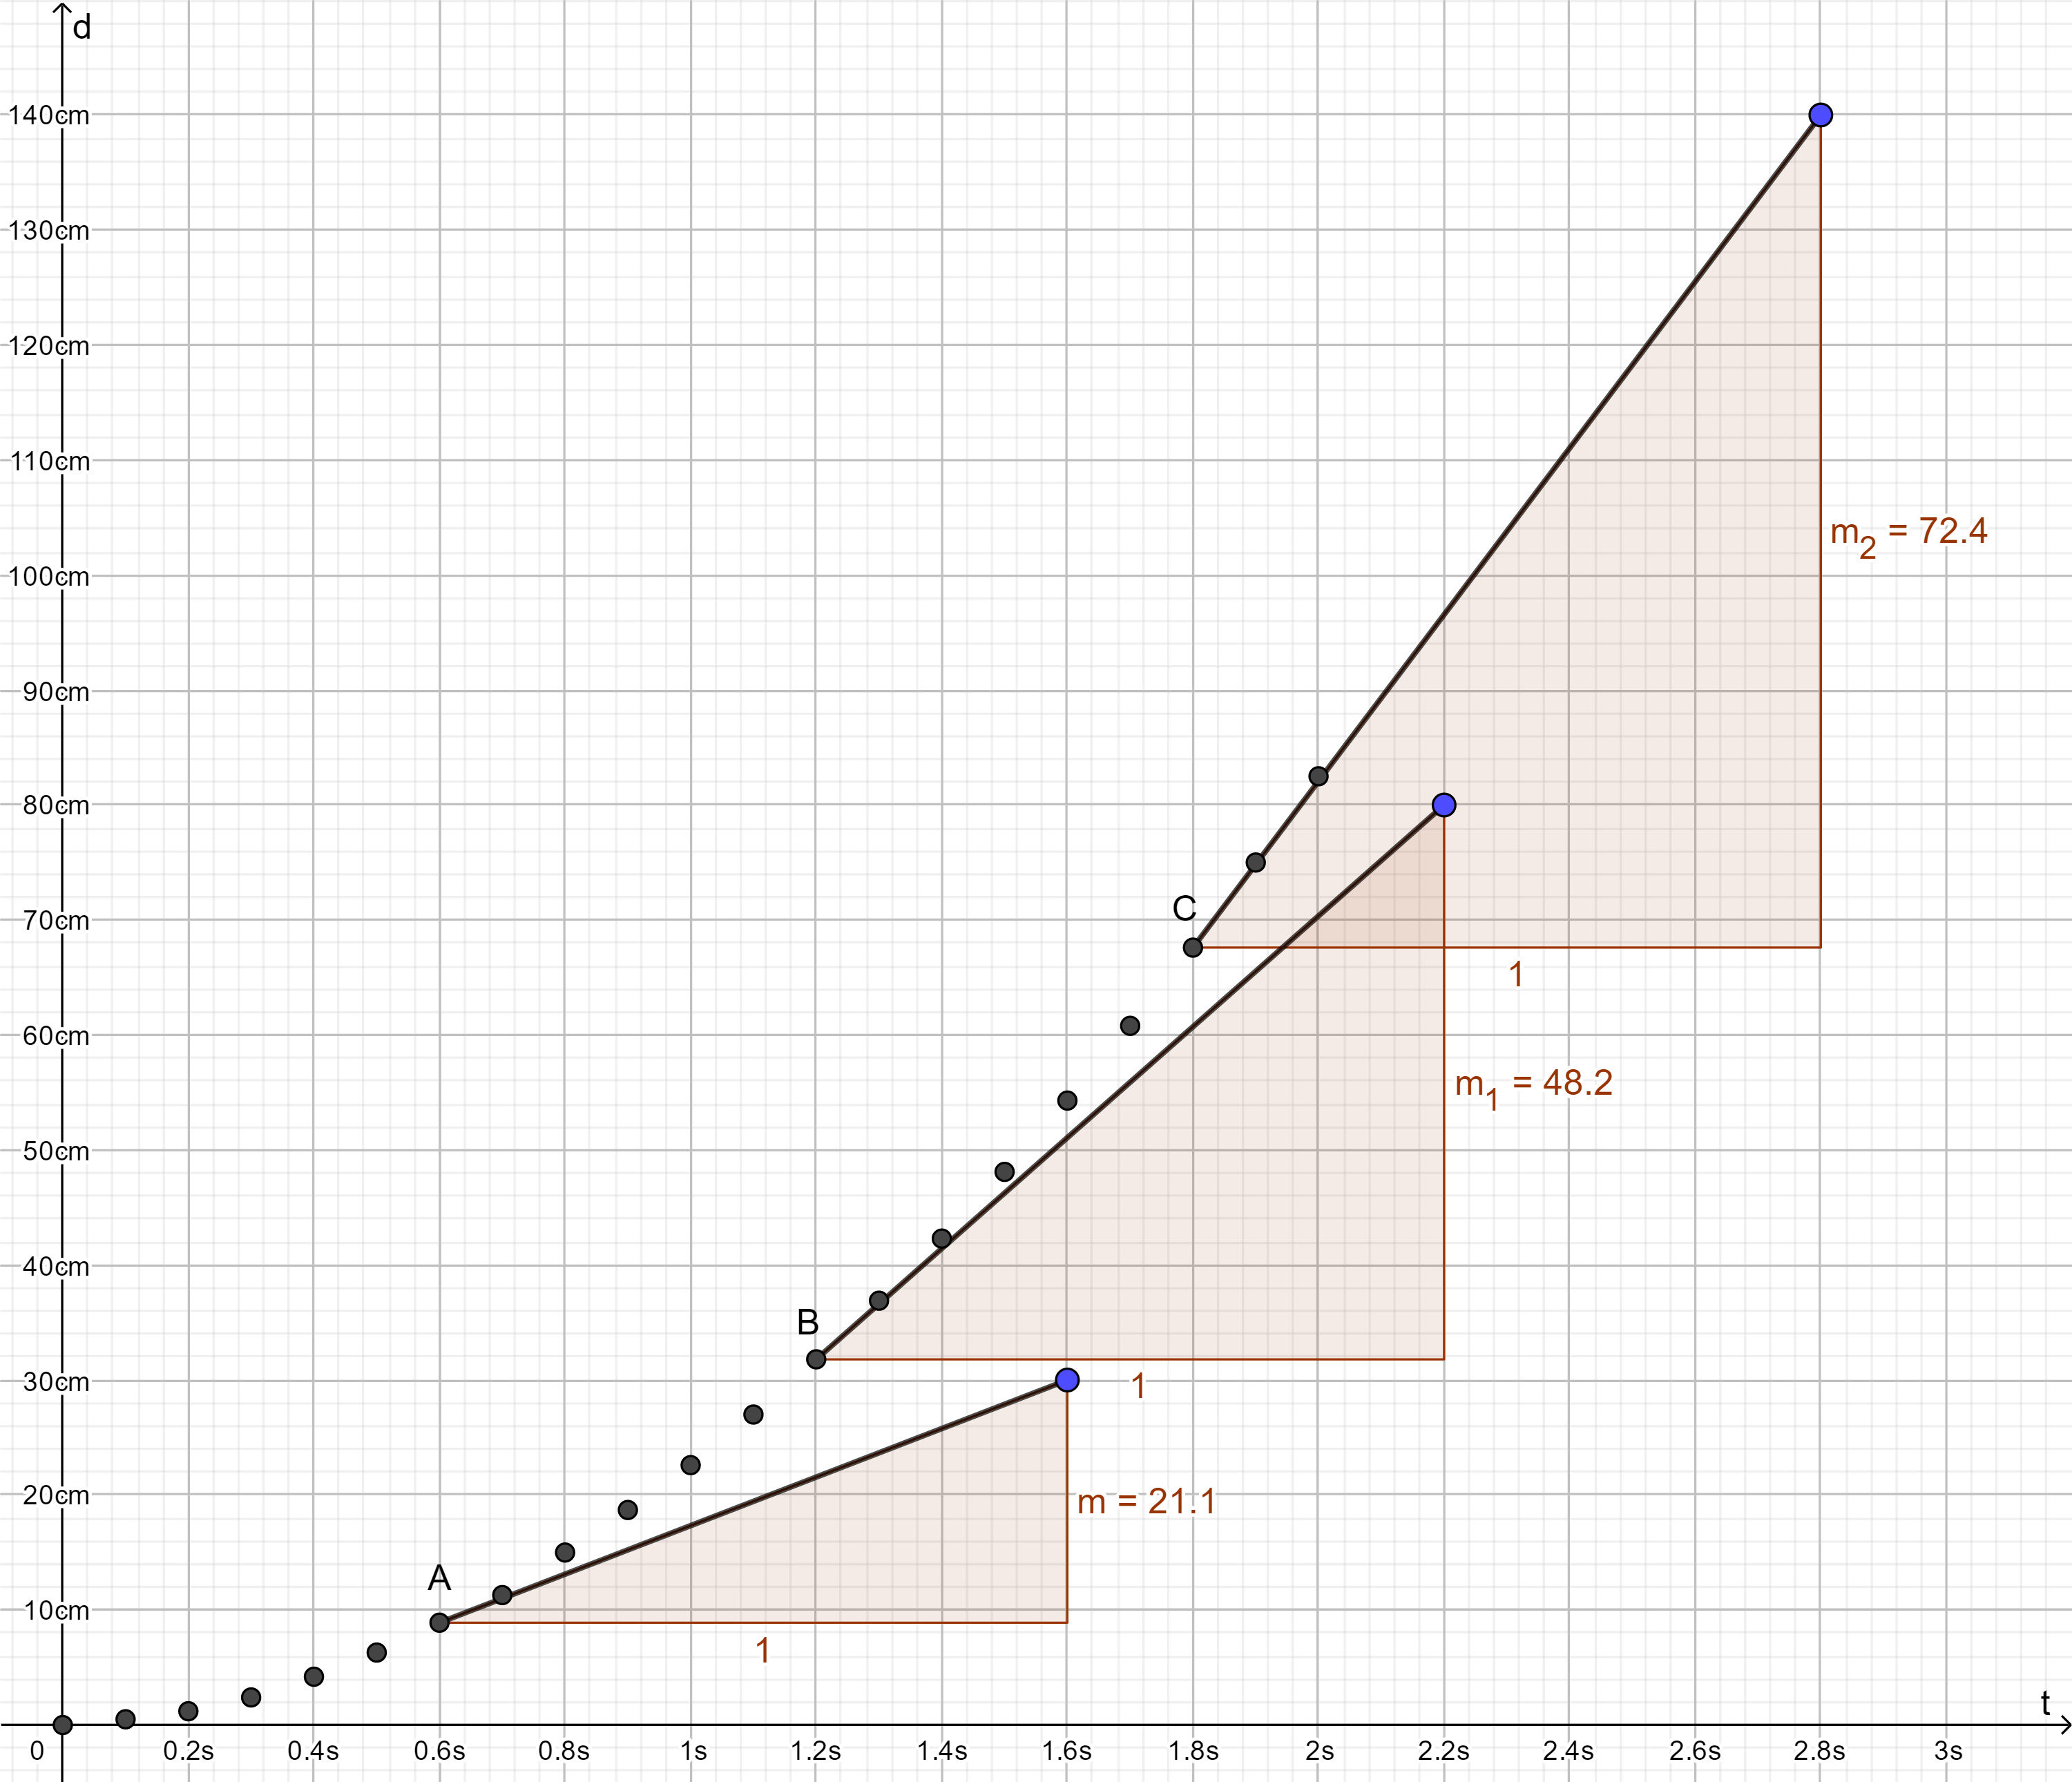
\includegraphics[scale=1.25]{LabReportImg/5TB-Tangents.png}
            \captionof*{figure}{Trial one}
        \end{minipage}
        \begin{minipage}{0.4\textwidth}
            \centering
            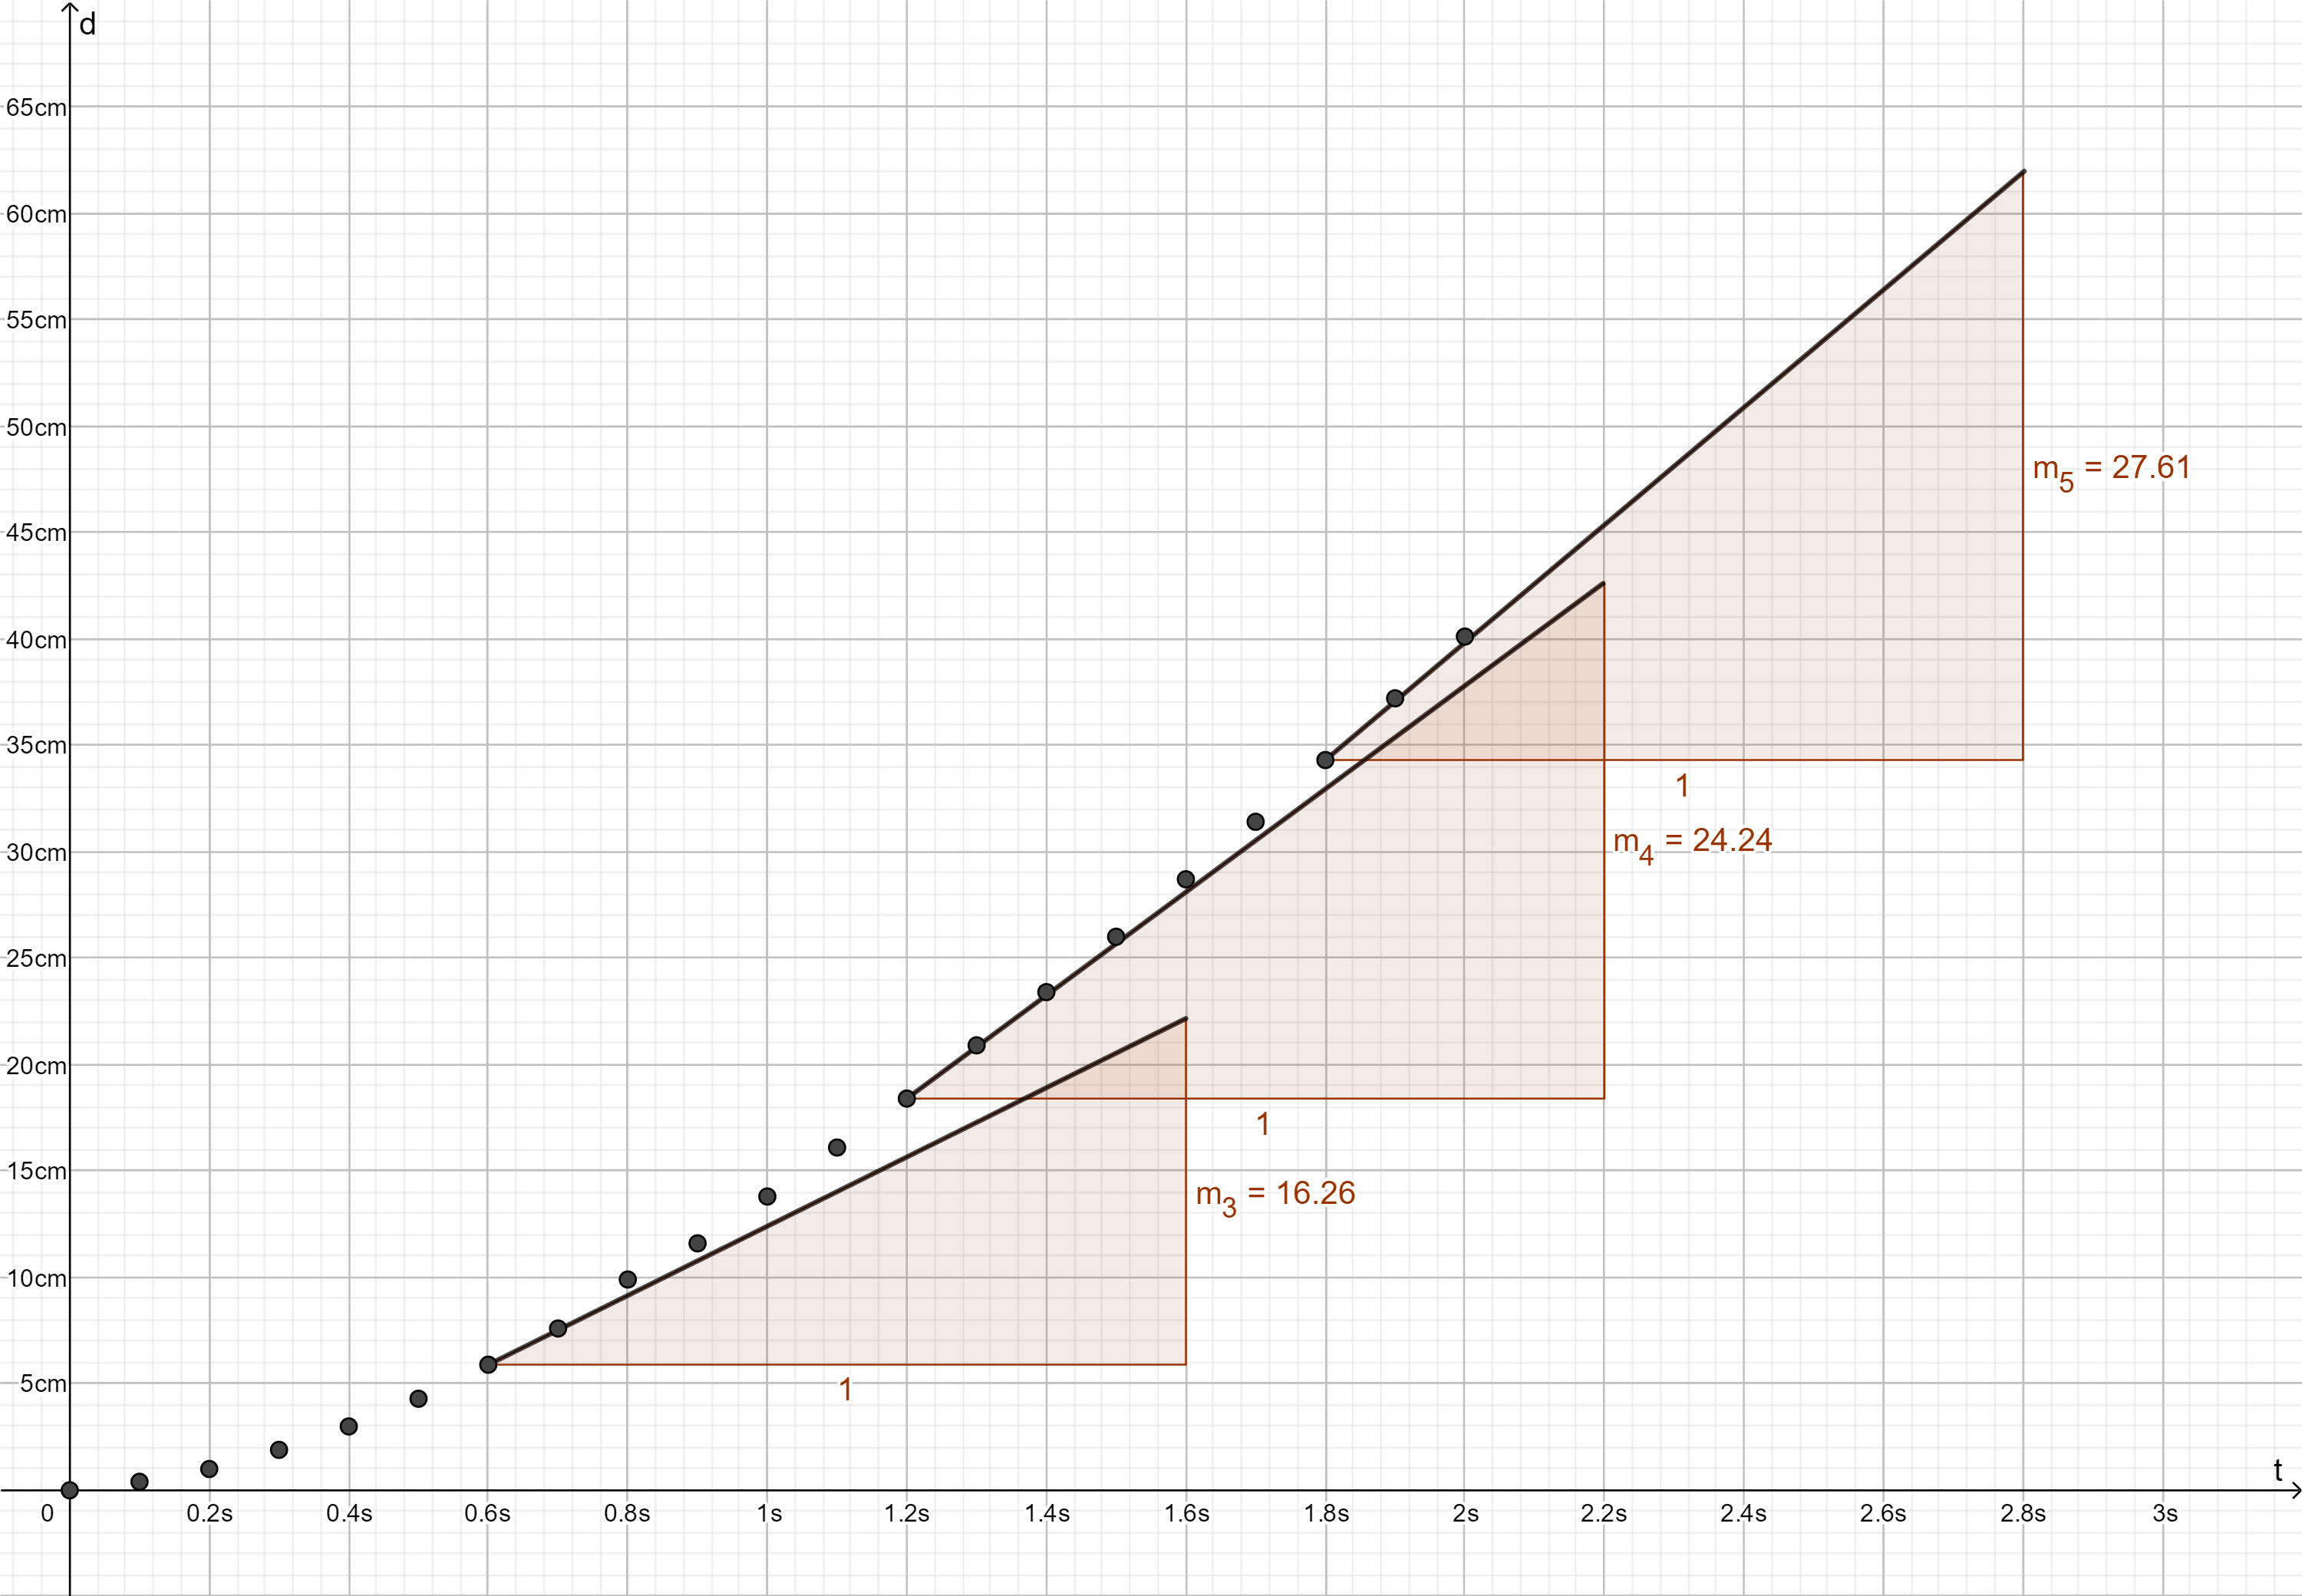
\includegraphics[scale=1.25]{LabReportImg/3TB-Tangents.png}
            \captionof*{figure}{Trial two}
        \end{minipage}
        \caption{Tangents of both trials}
        \label{fig:Tangents}
    \end{figure}
    \item Calculate the slops of the tangents which equal the instantaneous velocities at these chosen specific times.
    \begin{itemize}
        \item The slopes are calculated in Figure \ref{fig:Tangents}, as the $\Delta x$ for each tangent "triangle" is 1, meaning the $\Delta y$ is the slope of the tangent.
    \end{itemize}
    \item Record these velocities in a table indicating the time and the velocity at that particular time to plot a velocity-time graph for every trial.
    \begin{center}
        \begin{tabular}{c|c @{\hspace{5em}} c|c}
            \multicolumn{2}{c}{Trial 1}&\multicolumn{2}{c}{Trial 2}\\
            \hline
            Time&Position&Time&Position\\
            0.6&0.212&0.6&0.163\\
            1.2&0.482&1.2&0.242\\
            1.8&0.724&1.8&0.276\\
        \end{tabular}
    \end{center}
    \begin{figure}[H]
        \centering
        \begin{minipage}{0.4\textwidth}
            \centering
            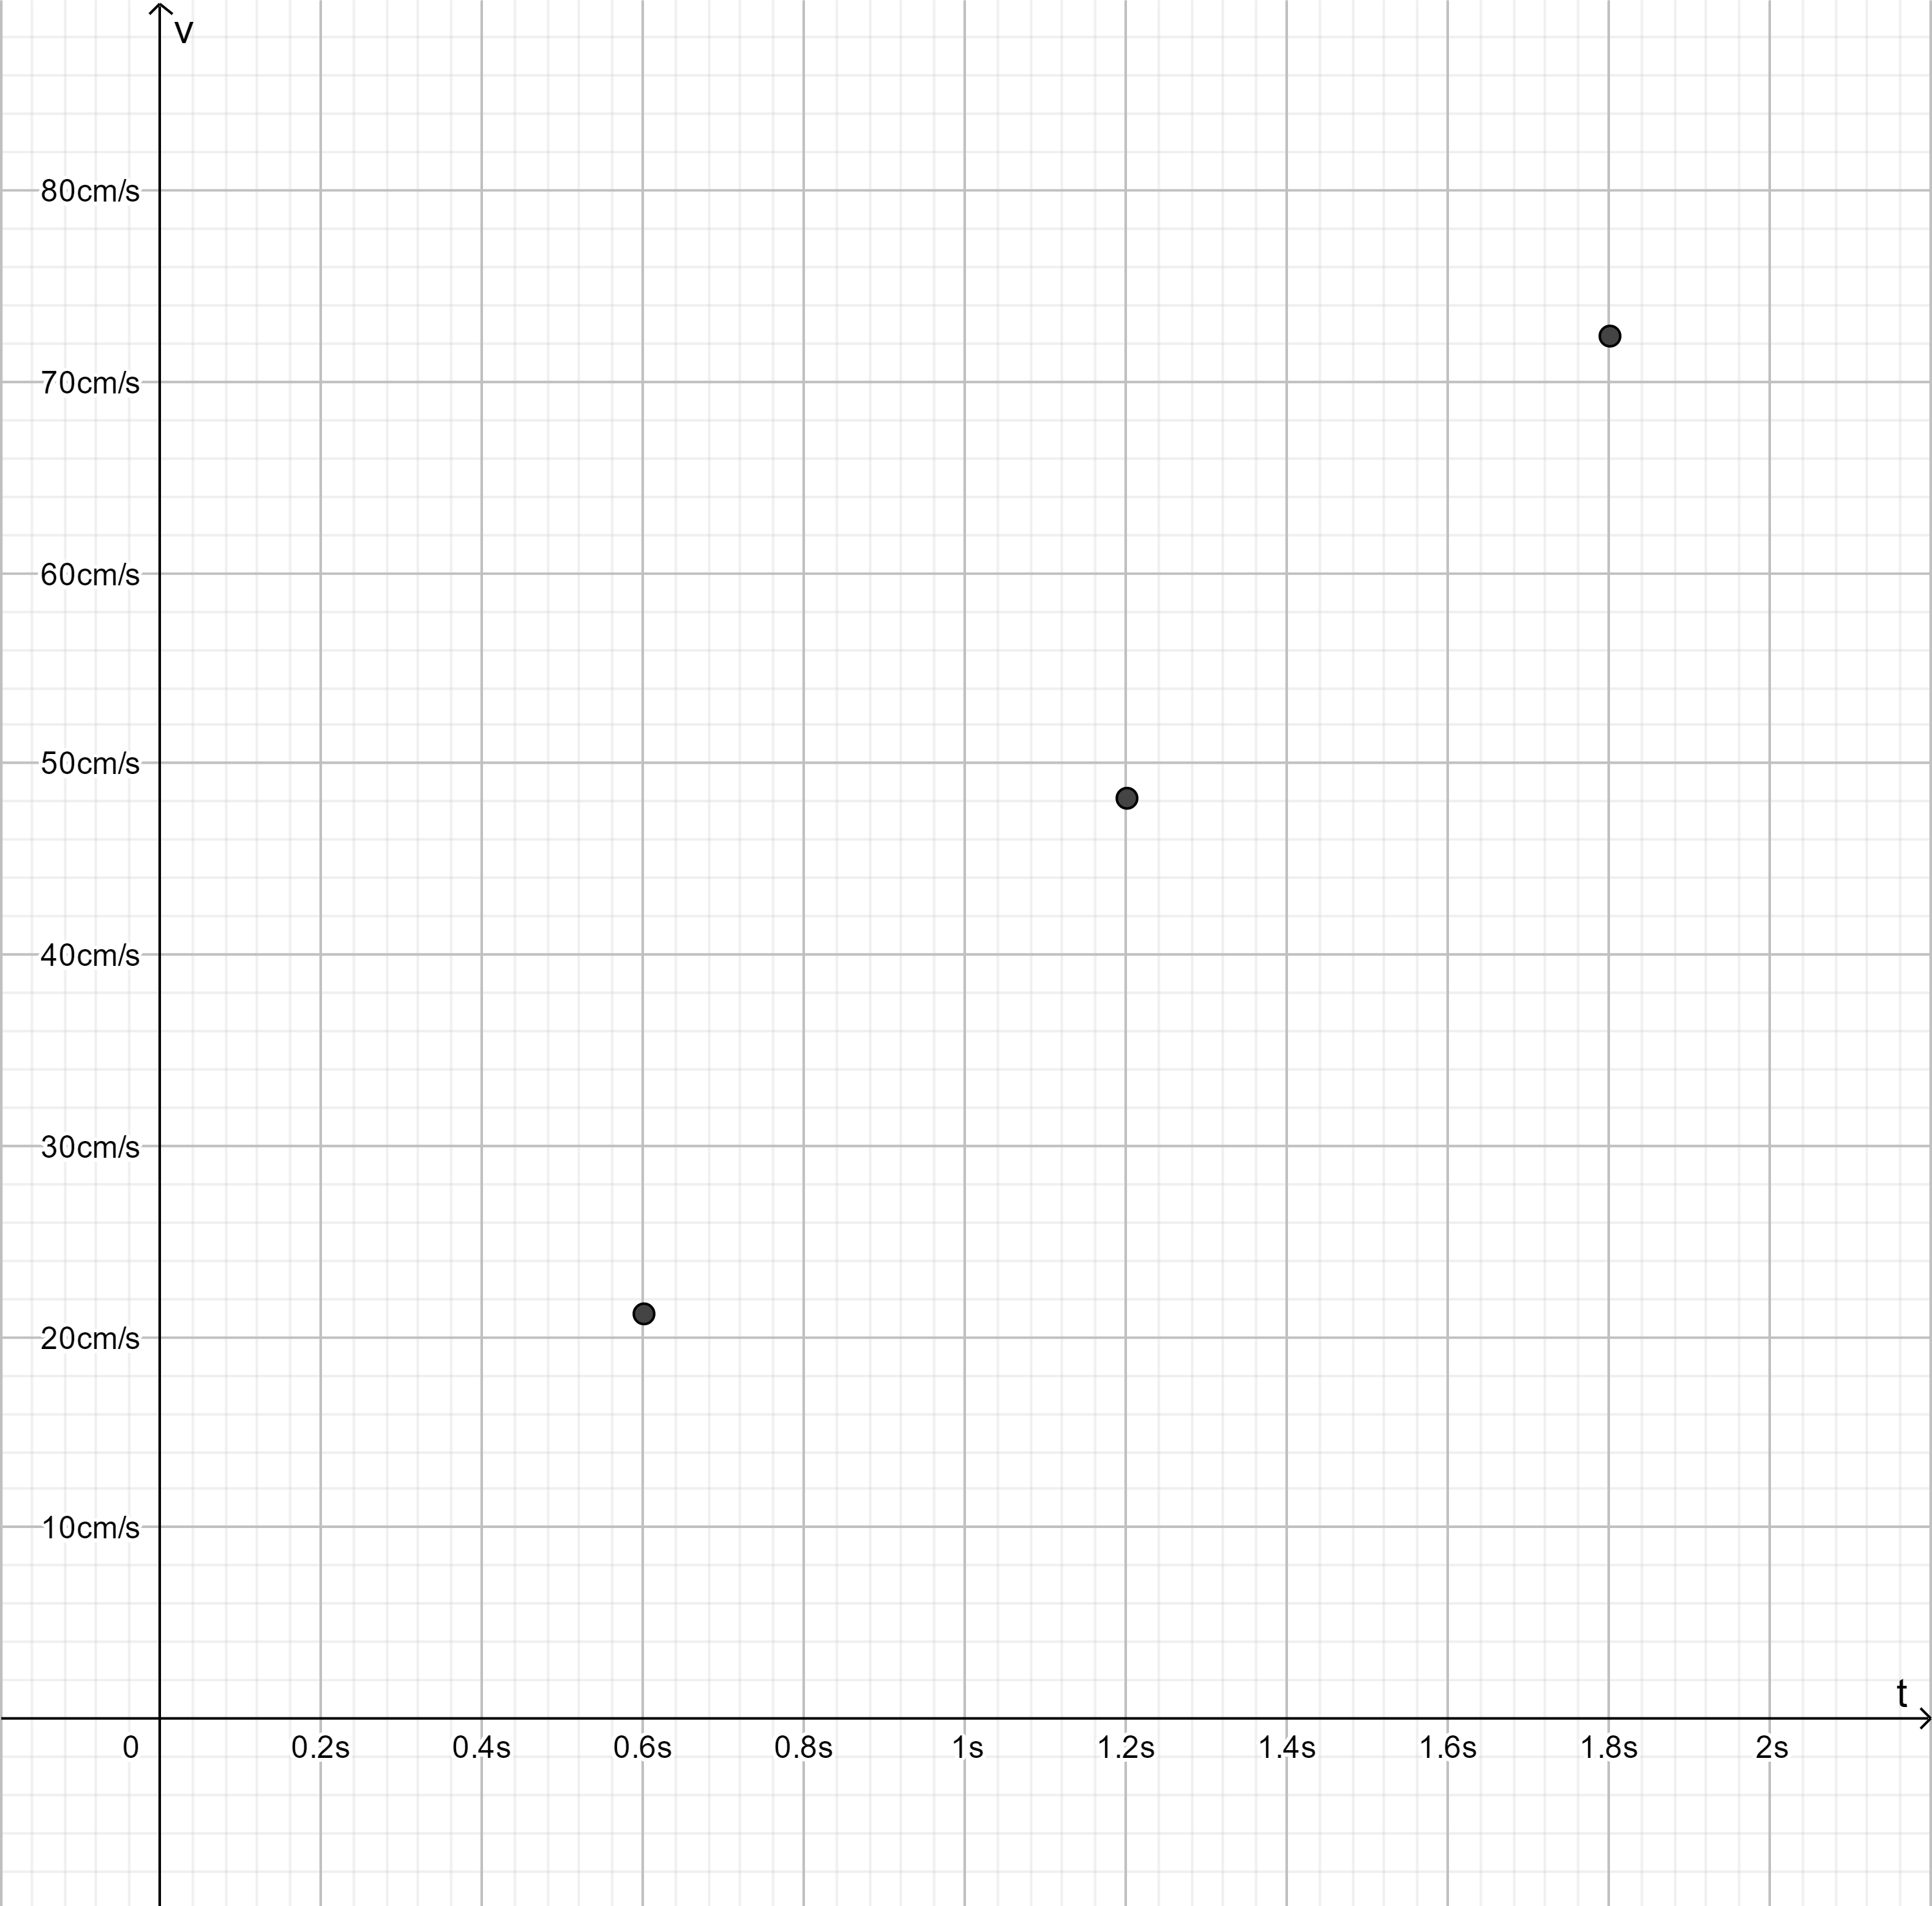
\includegraphics[scale=1.25]{LabReportImg/5TB-TangentPoints.png}
            \captionof*{figure}{Trial one}
            \label{fig:V-T Trail one}
        \end{minipage}
        \begin{minipage}{0.4\textwidth}
            \centering
            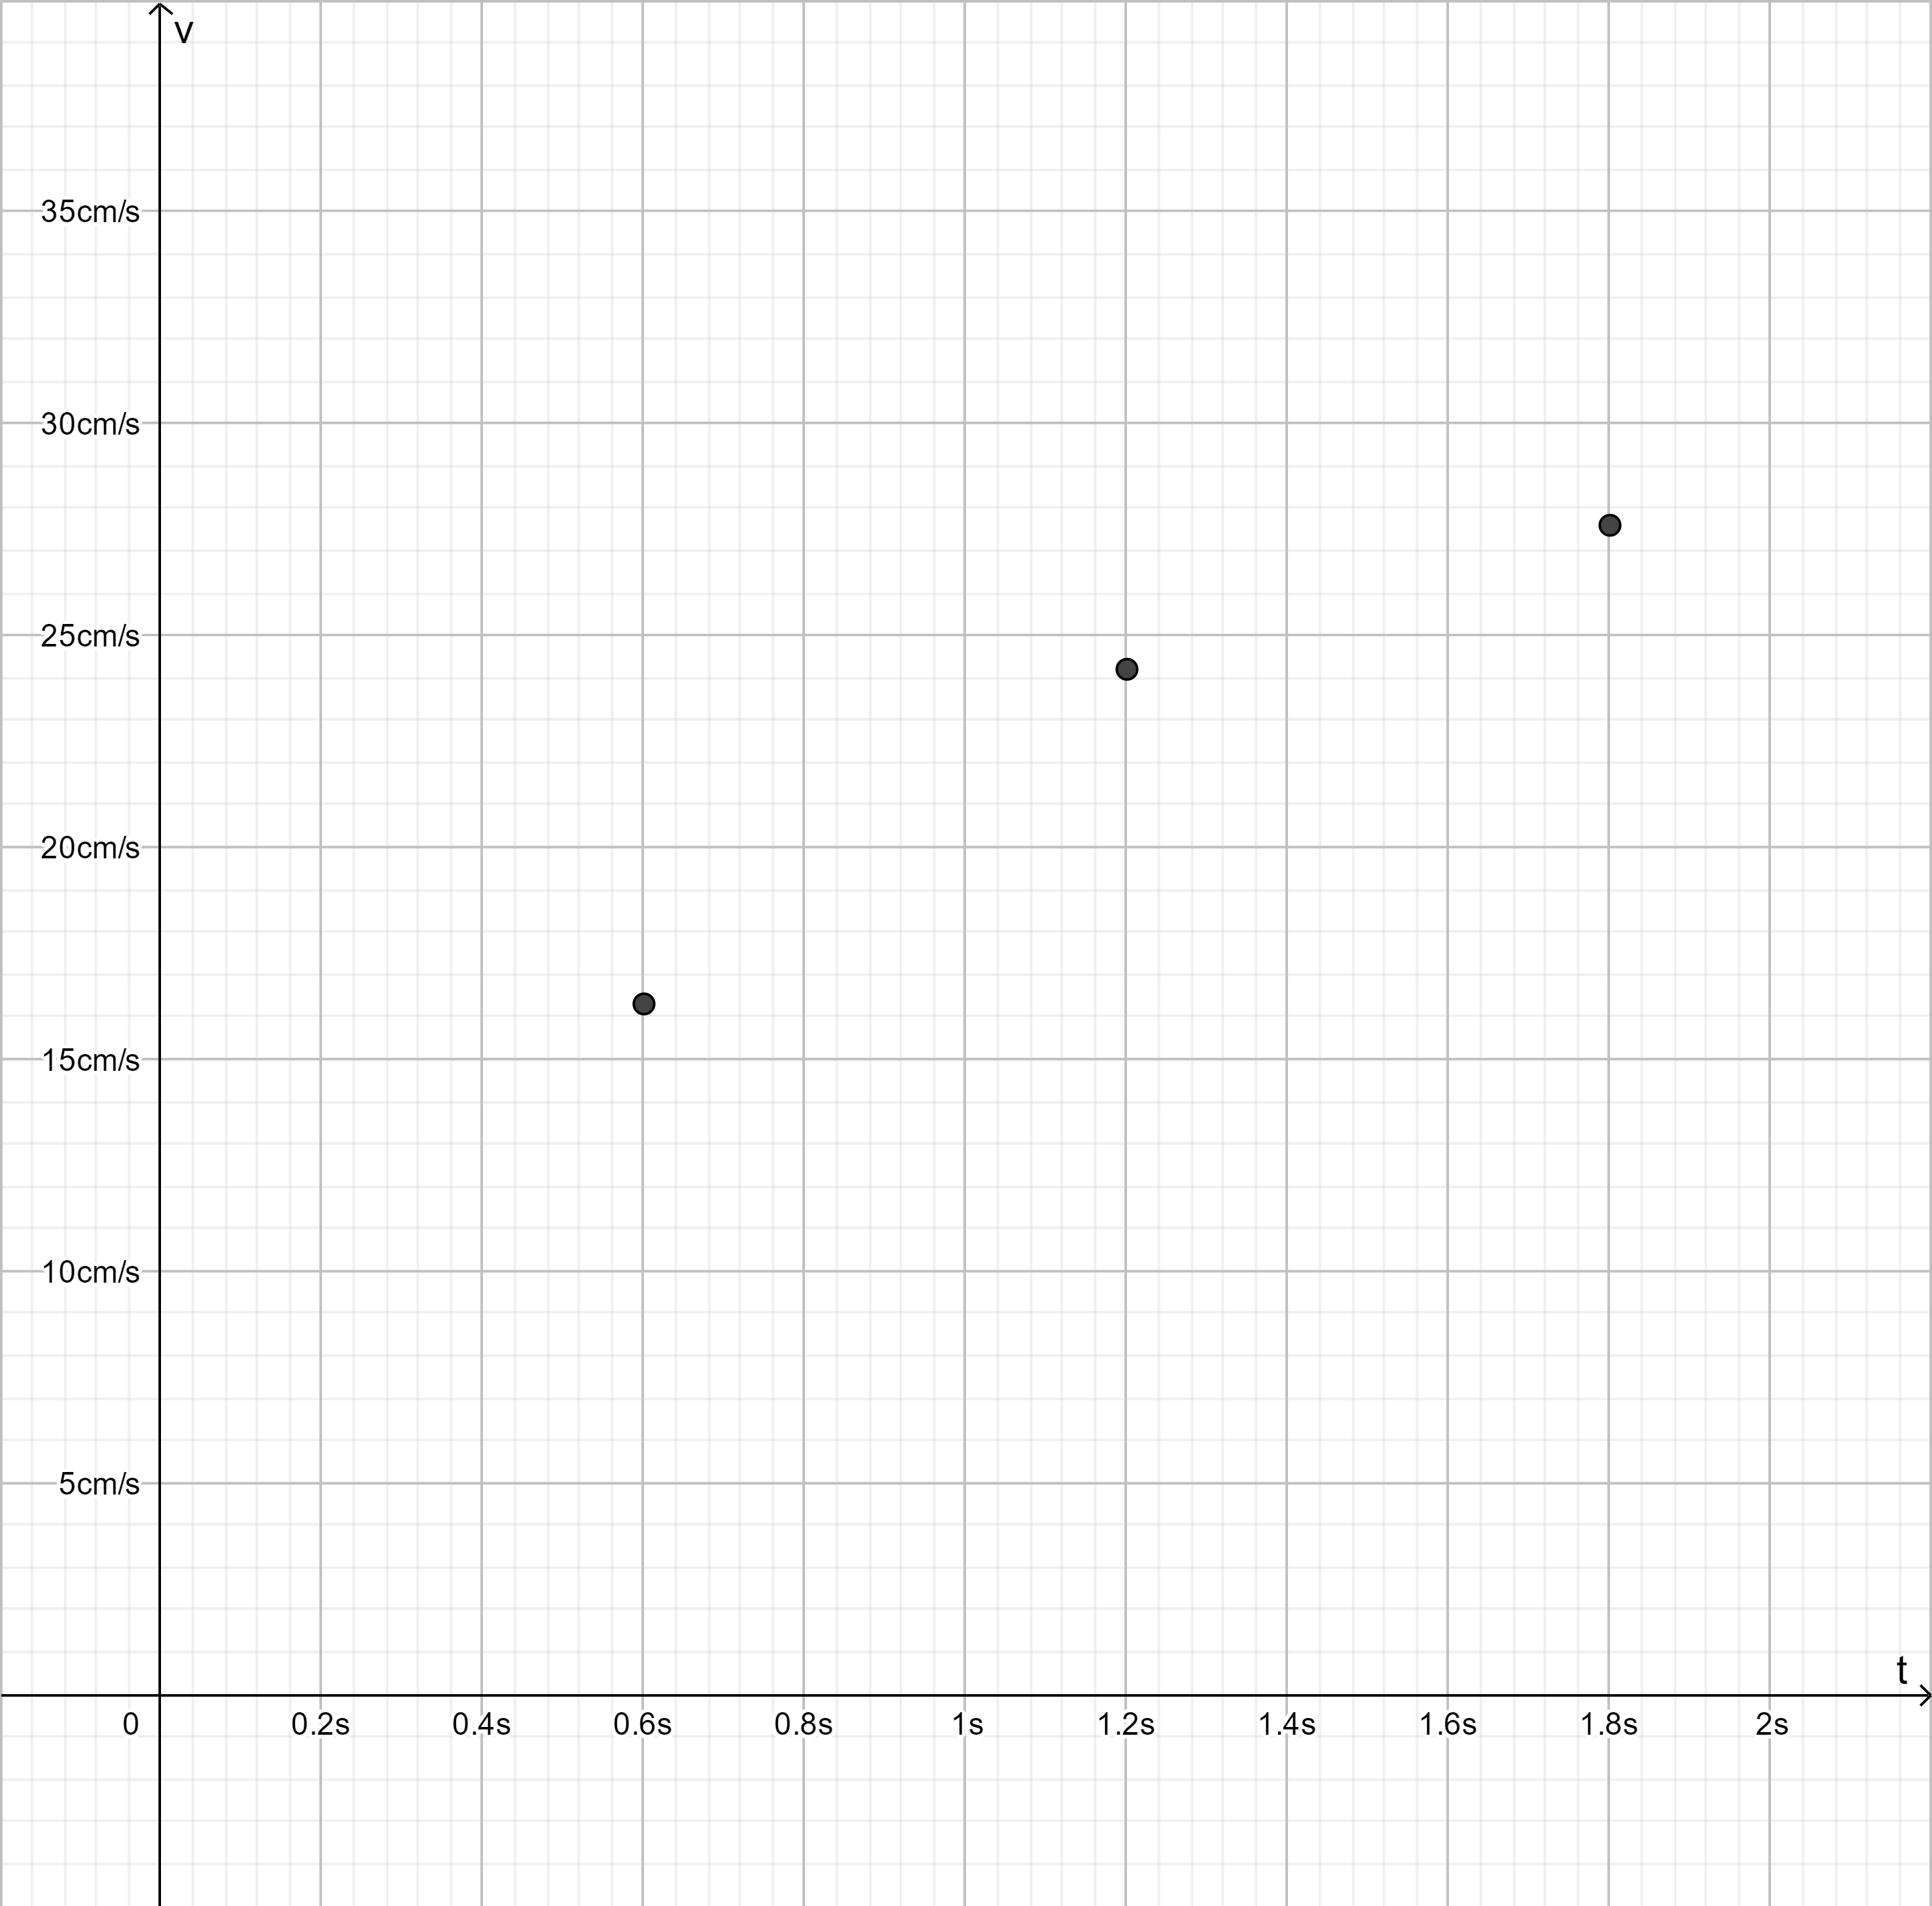
\includegraphics[scale=1.25]{LabReportImg/3TB-TangentPoints.png}
            \captionof*{figure}{Trial two}
            \label{fig:V-T Trail two}
        \end{minipage}
    \end{figure}
    \item Draw a line of best fit for every graph that best approximates the relationship.
    \begin{figure}[H]
        \centering
        \begin{minipage}{0.4\textwidth}
            \centering
            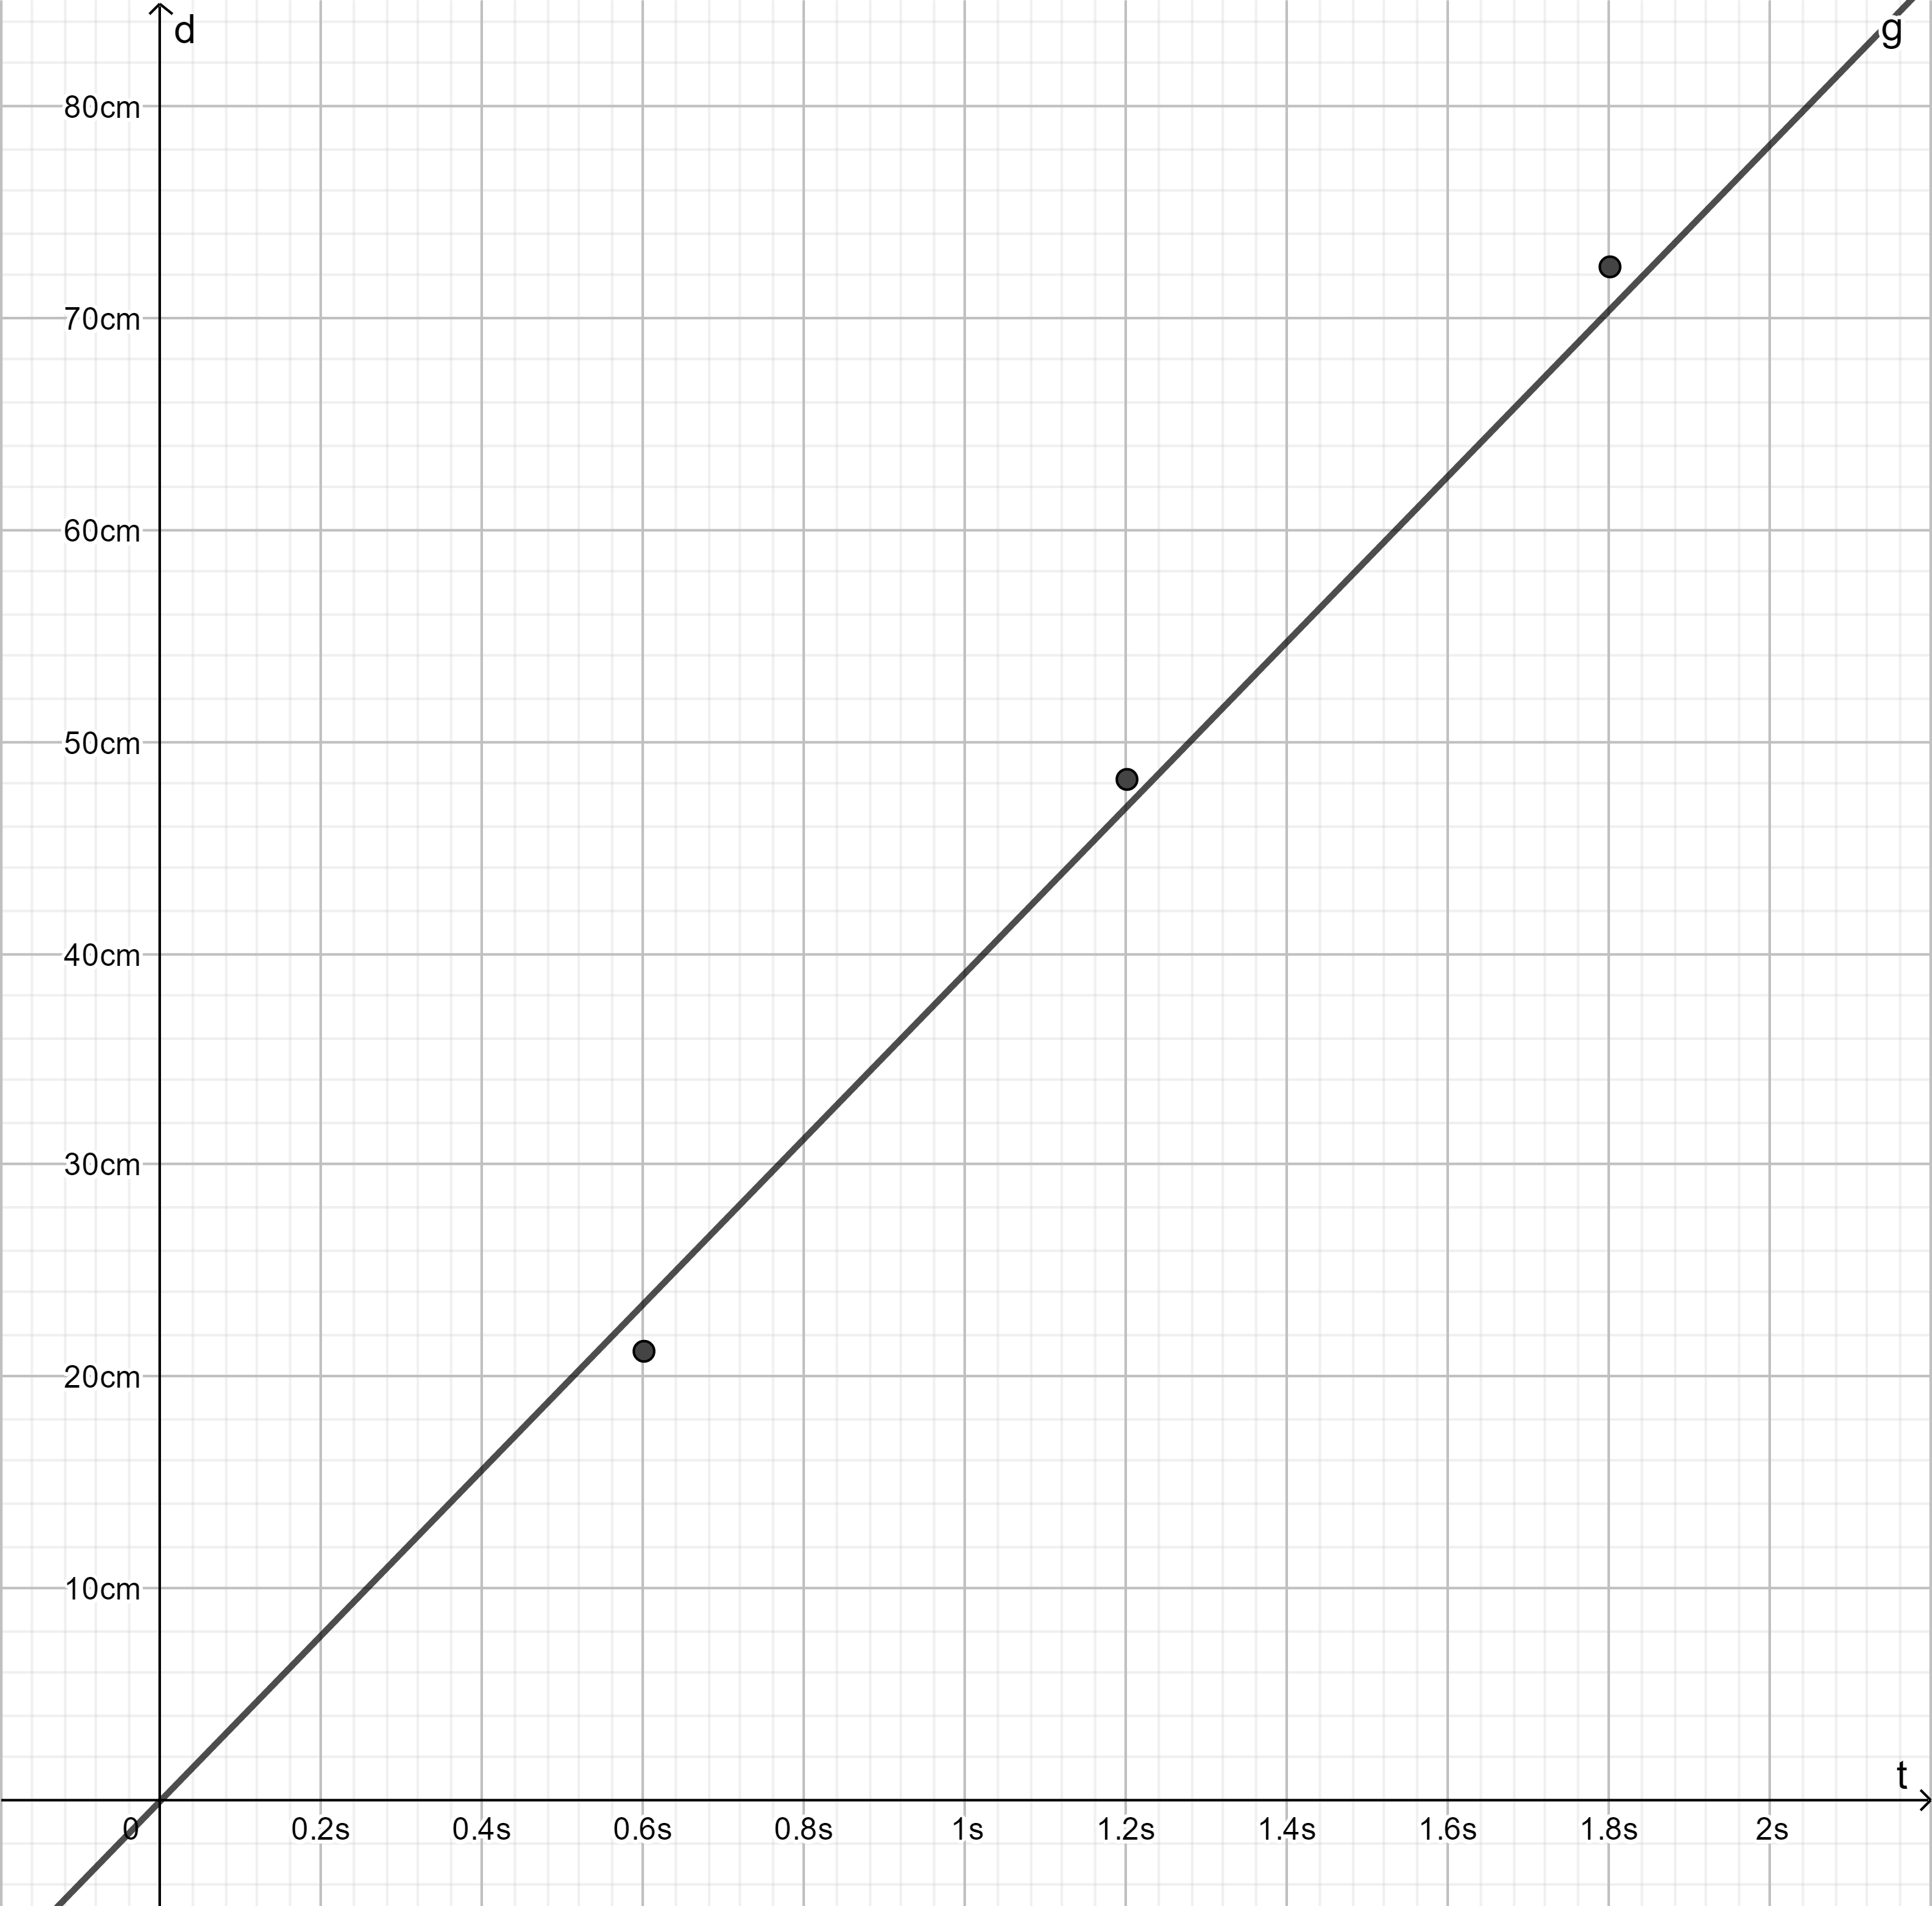
\includegraphics[scale=1.25]{LabReportImg/5TB-TangentLine.png}
            \captionof*{figure}{Trial one}
        \end{minipage}
        \begin{minipage}{0.4\textwidth}
            \centering
            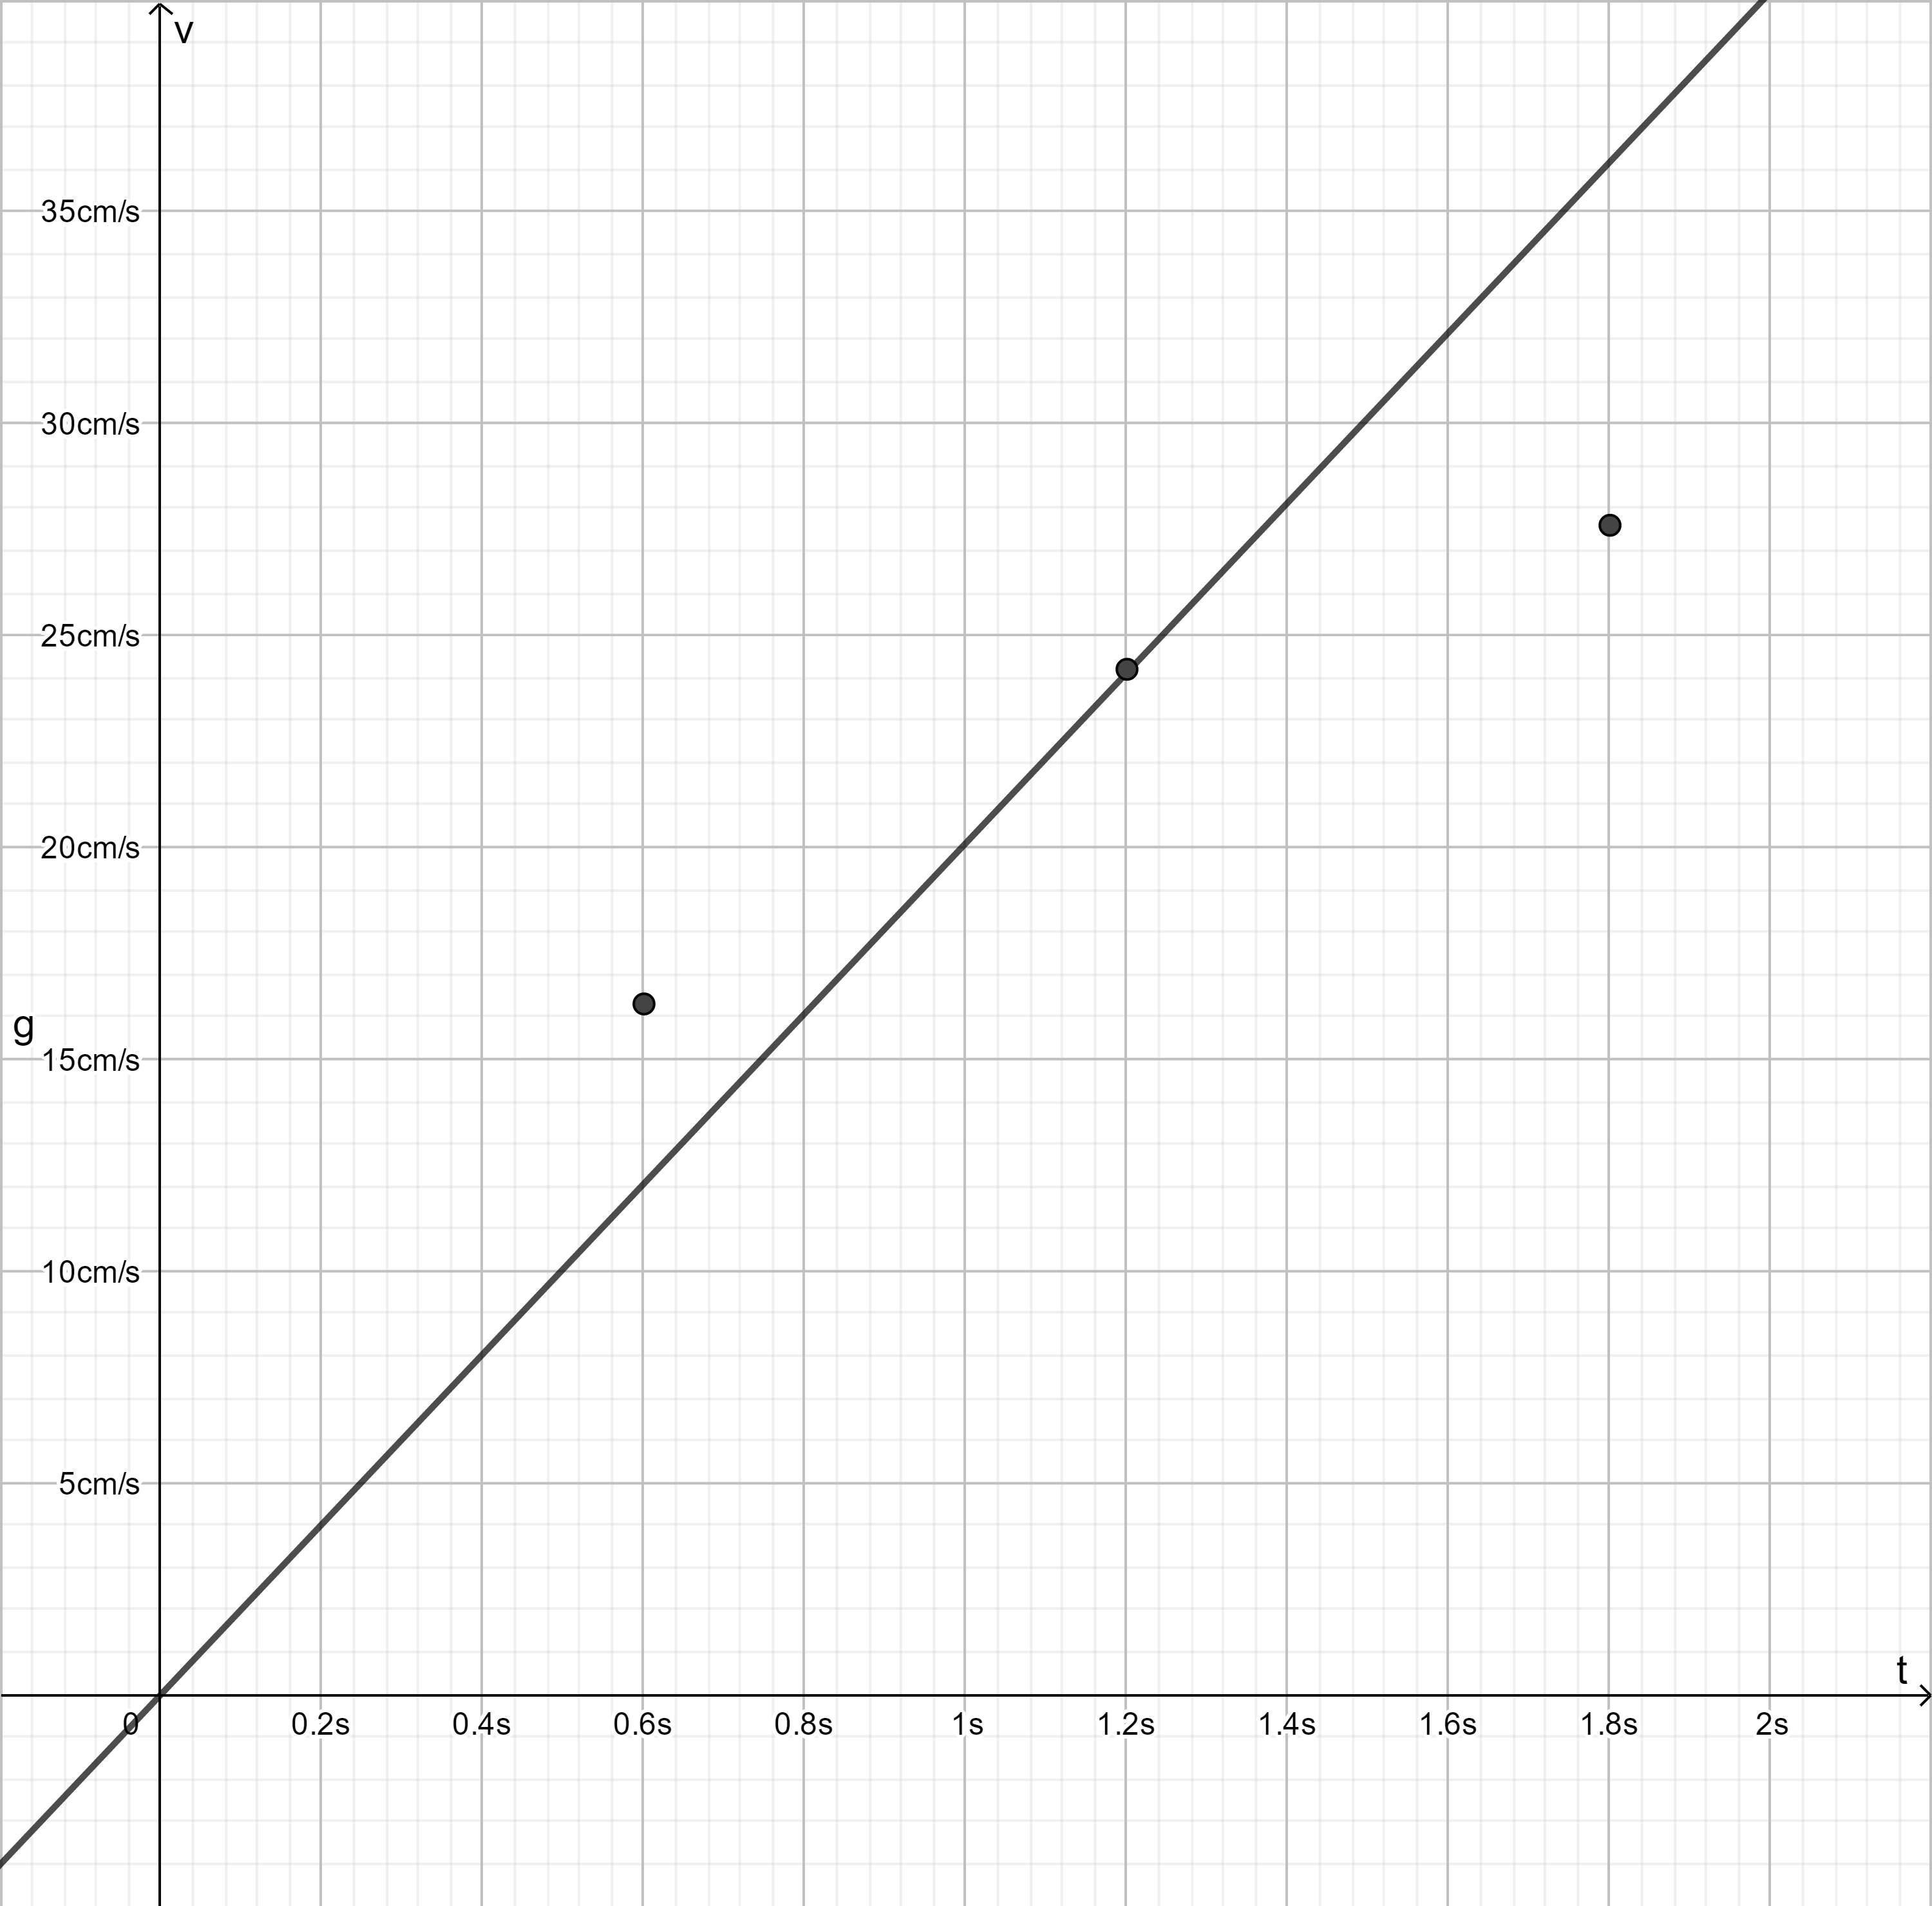
\includegraphics[scale=1.25]{LabReportImg/3TB-TangentLine.png}
            \captionof*{figure}{Trial two}
        \end{minipage}
    \end{figure}
    \item Calculate the slope of the velocity-time graph to determine the average acceleration ($\vec{a}$) for every graph.
    \begin{figure}[H]
        \centering
        \begin{minipage}{0.4\textwidth}
            \centering
            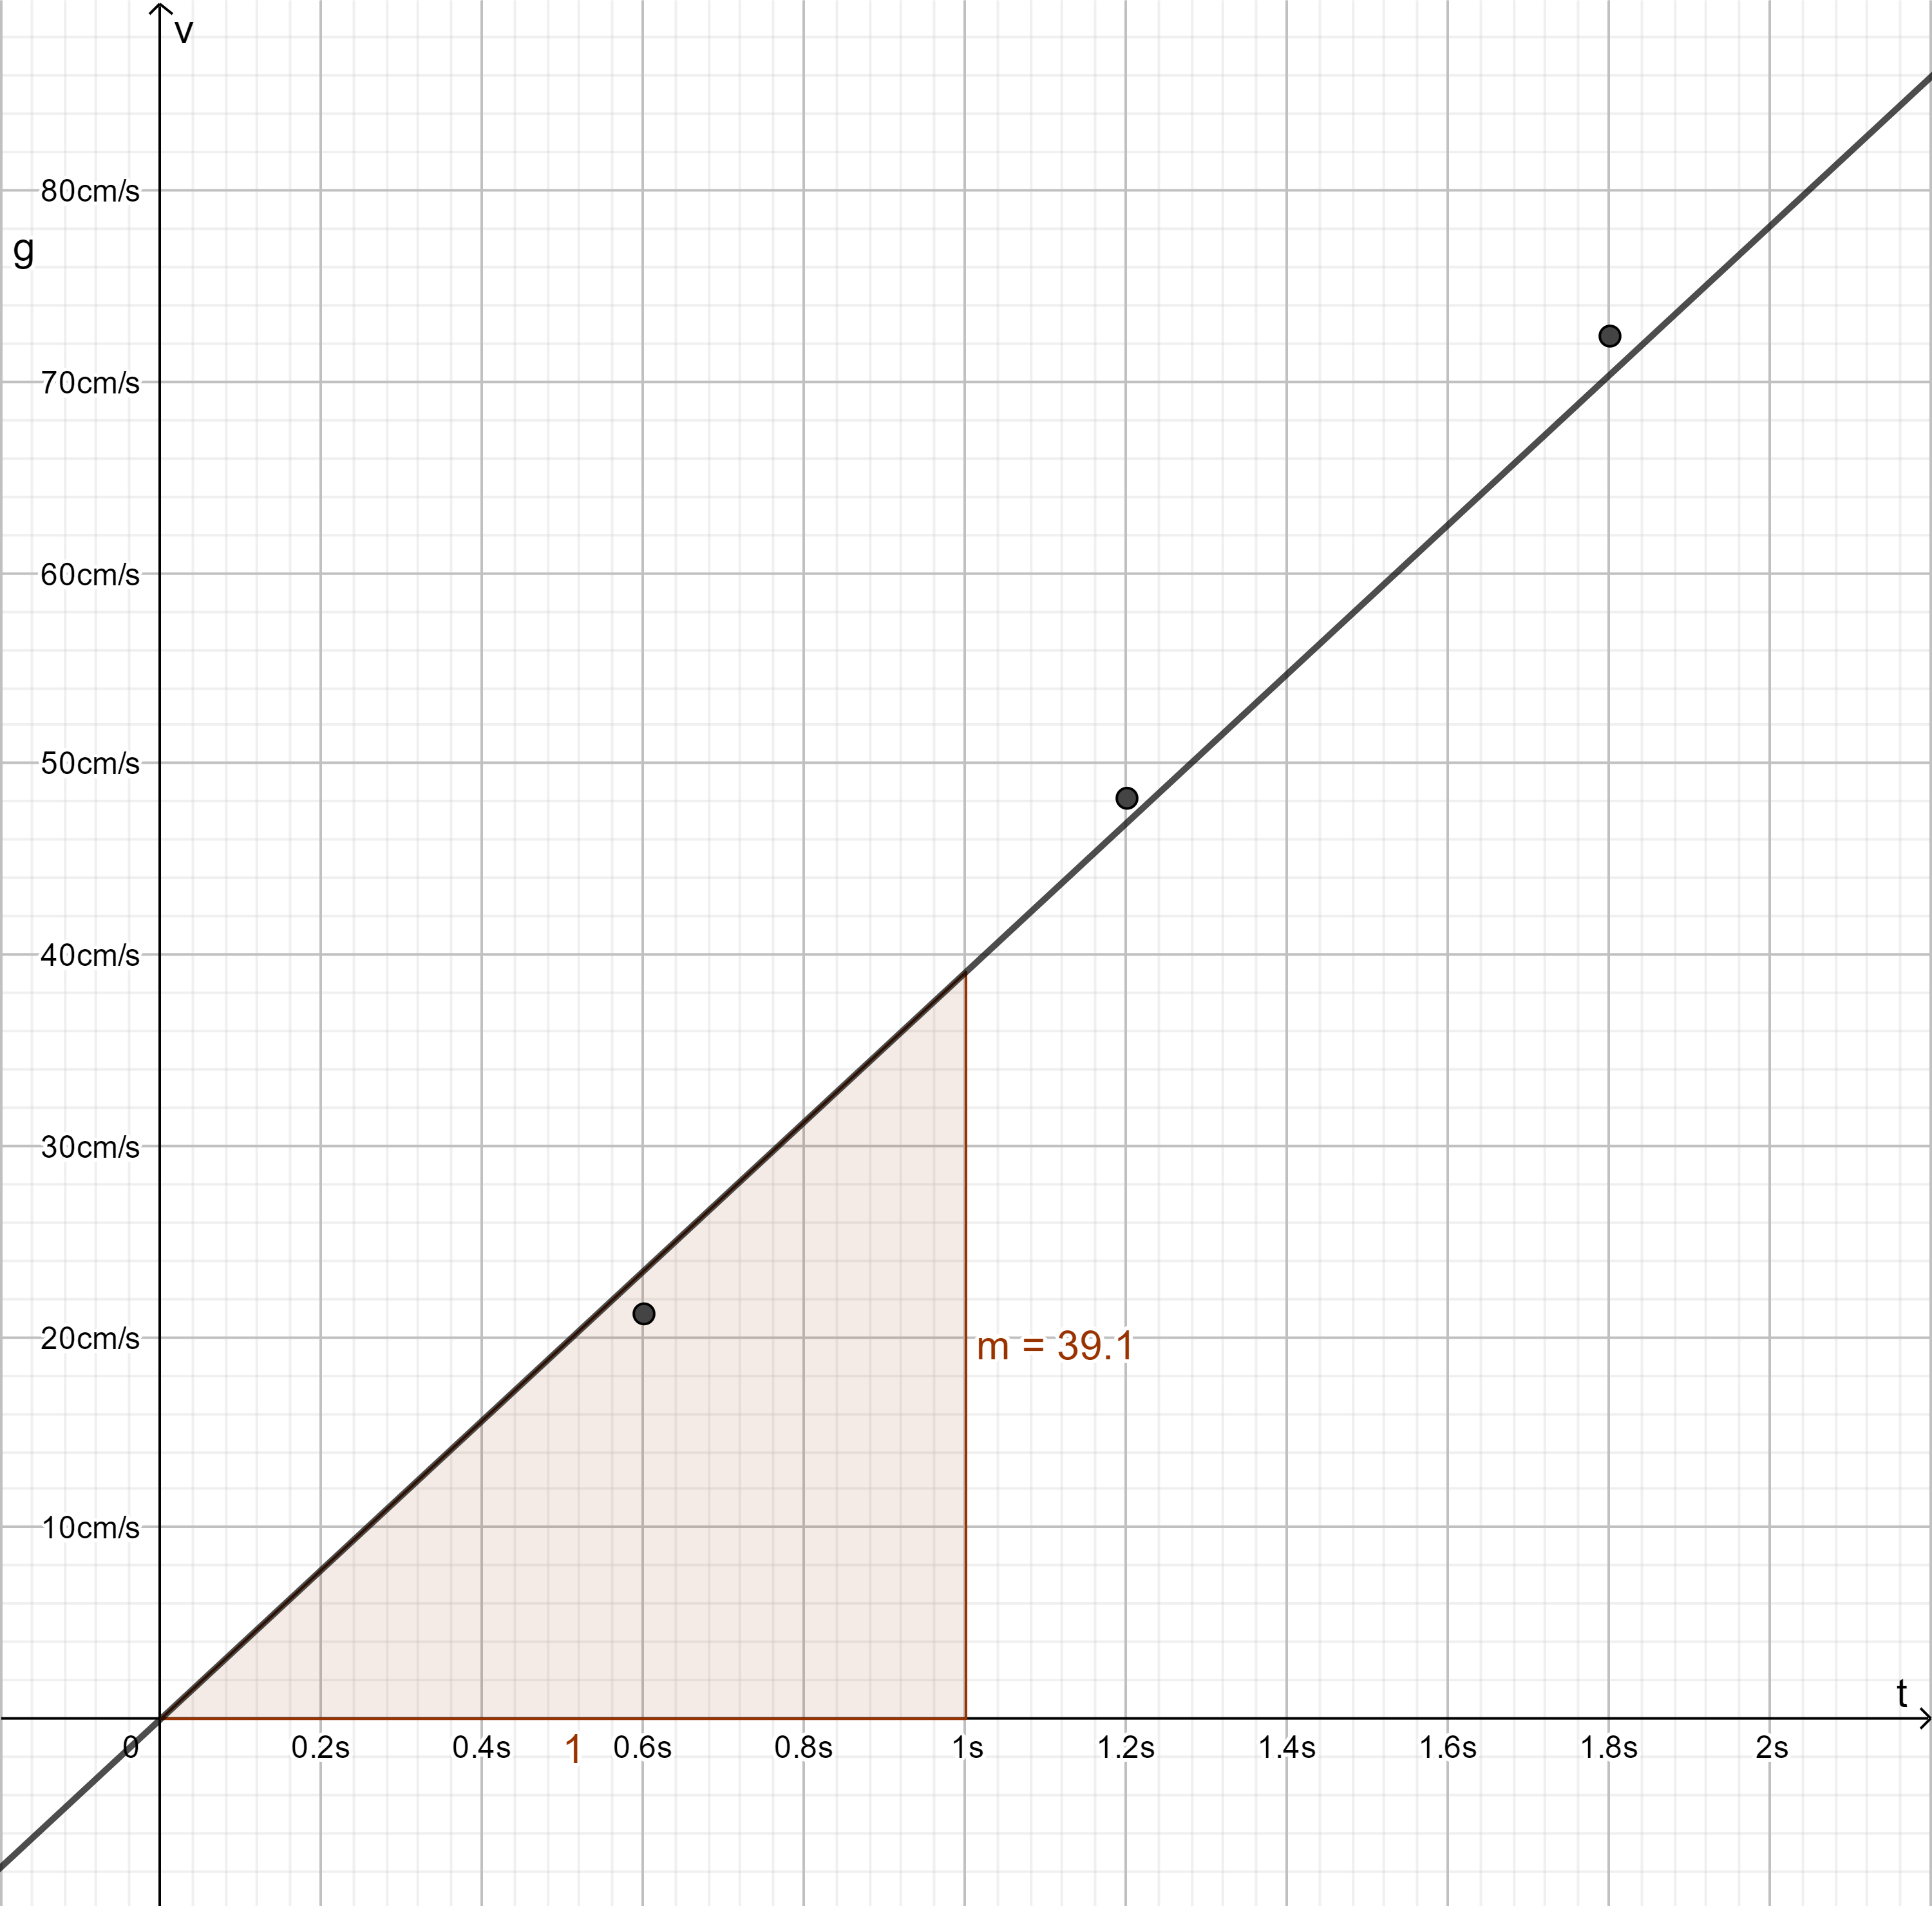
\includegraphics[scale=1.25]{LabReportImg/5TB-TangentSlope.png}
            \captionof*{figure}{Trial one: $\Delta x=1$\newline$\Delta y=0.391$ $\vec{a}=slope=0.391$}
        \end{minipage}
        \begin{minipage}{0.4\textwidth}
            \centering
            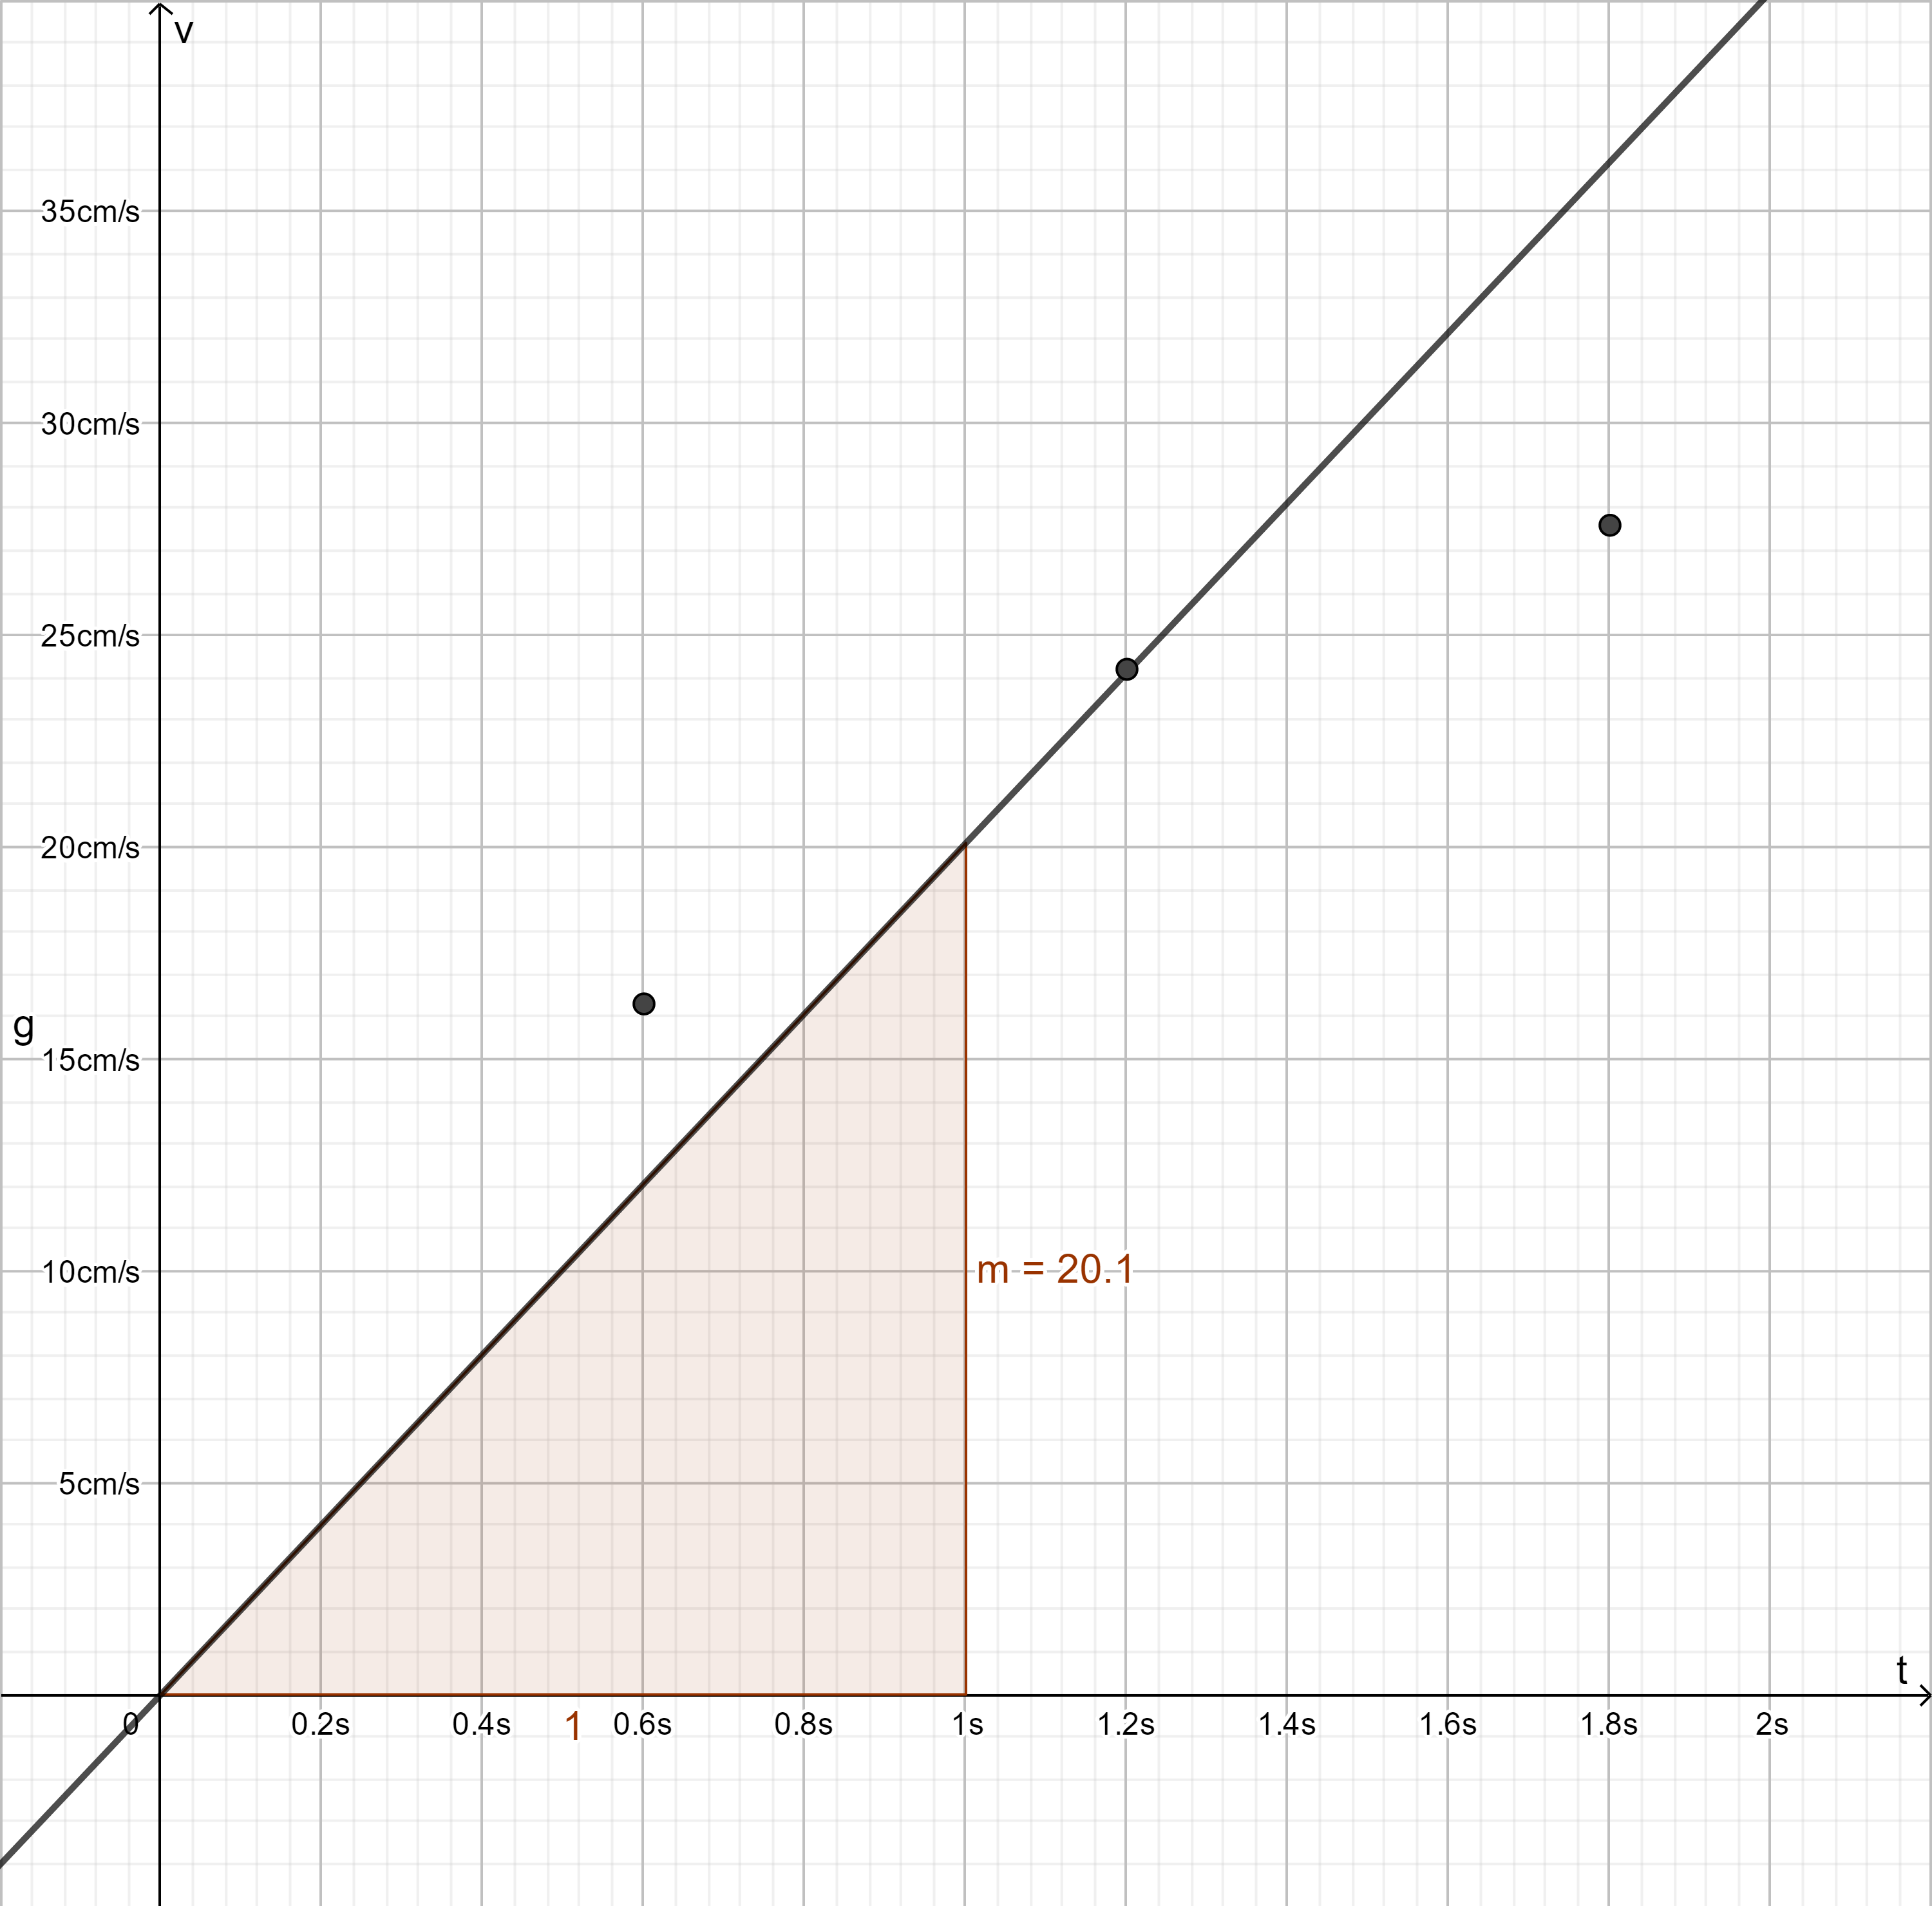
\includegraphics[scale=1.25]{LabReportImg/3TB-TangentSlope.png}
            \captionof*{figure}{Trial two: $\Delta x=1$\newline$\Delta y=0.201$ $\vec{a}=slope=0.201$}
        \end{minipage}
    \end{figure}
    \item Draw a-t graphs for the two trials.
    
    \begin{figure}[H]
        \centering
        \begin{minipage}{0.4\textwidth}
            \centering
            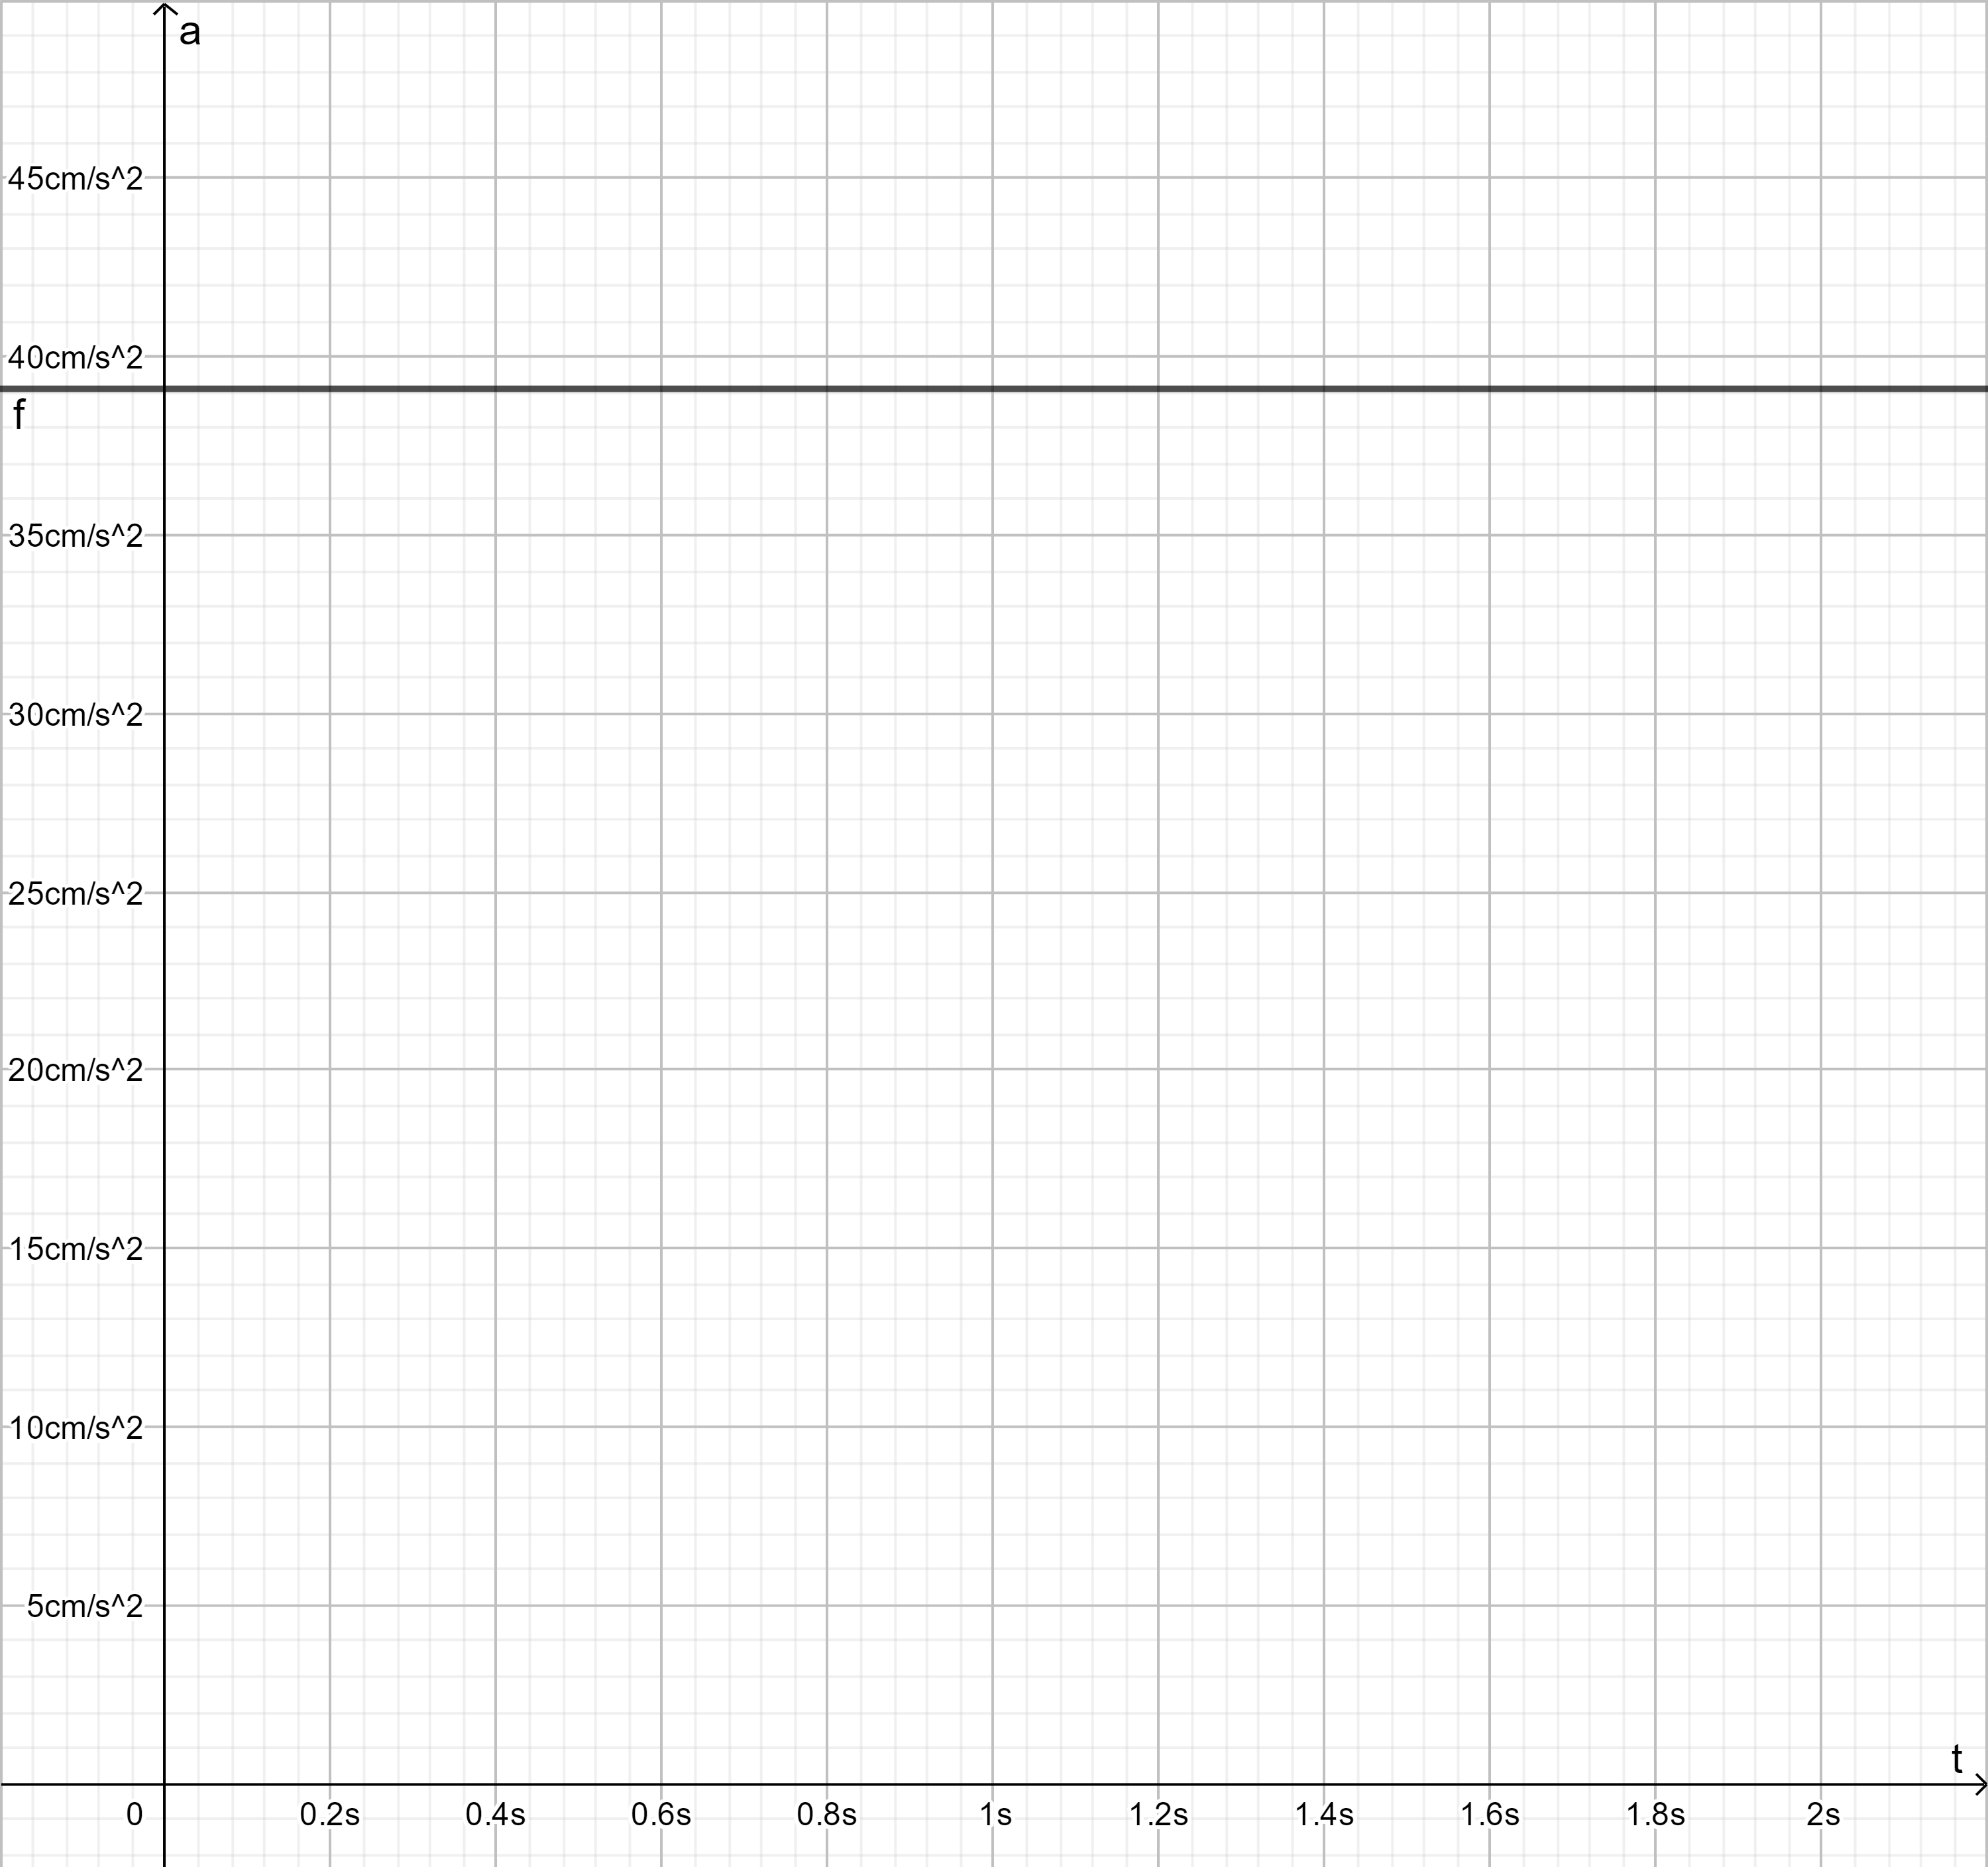
\includegraphics[scale=1.25]{LabReportImg/5TB-Acceleration.png}
            \captionof*{figure}{Trial one: $\vec{a}=0.391$}
        \end{minipage}
        \begin{minipage}{0.4\textwidth}
            \centering
            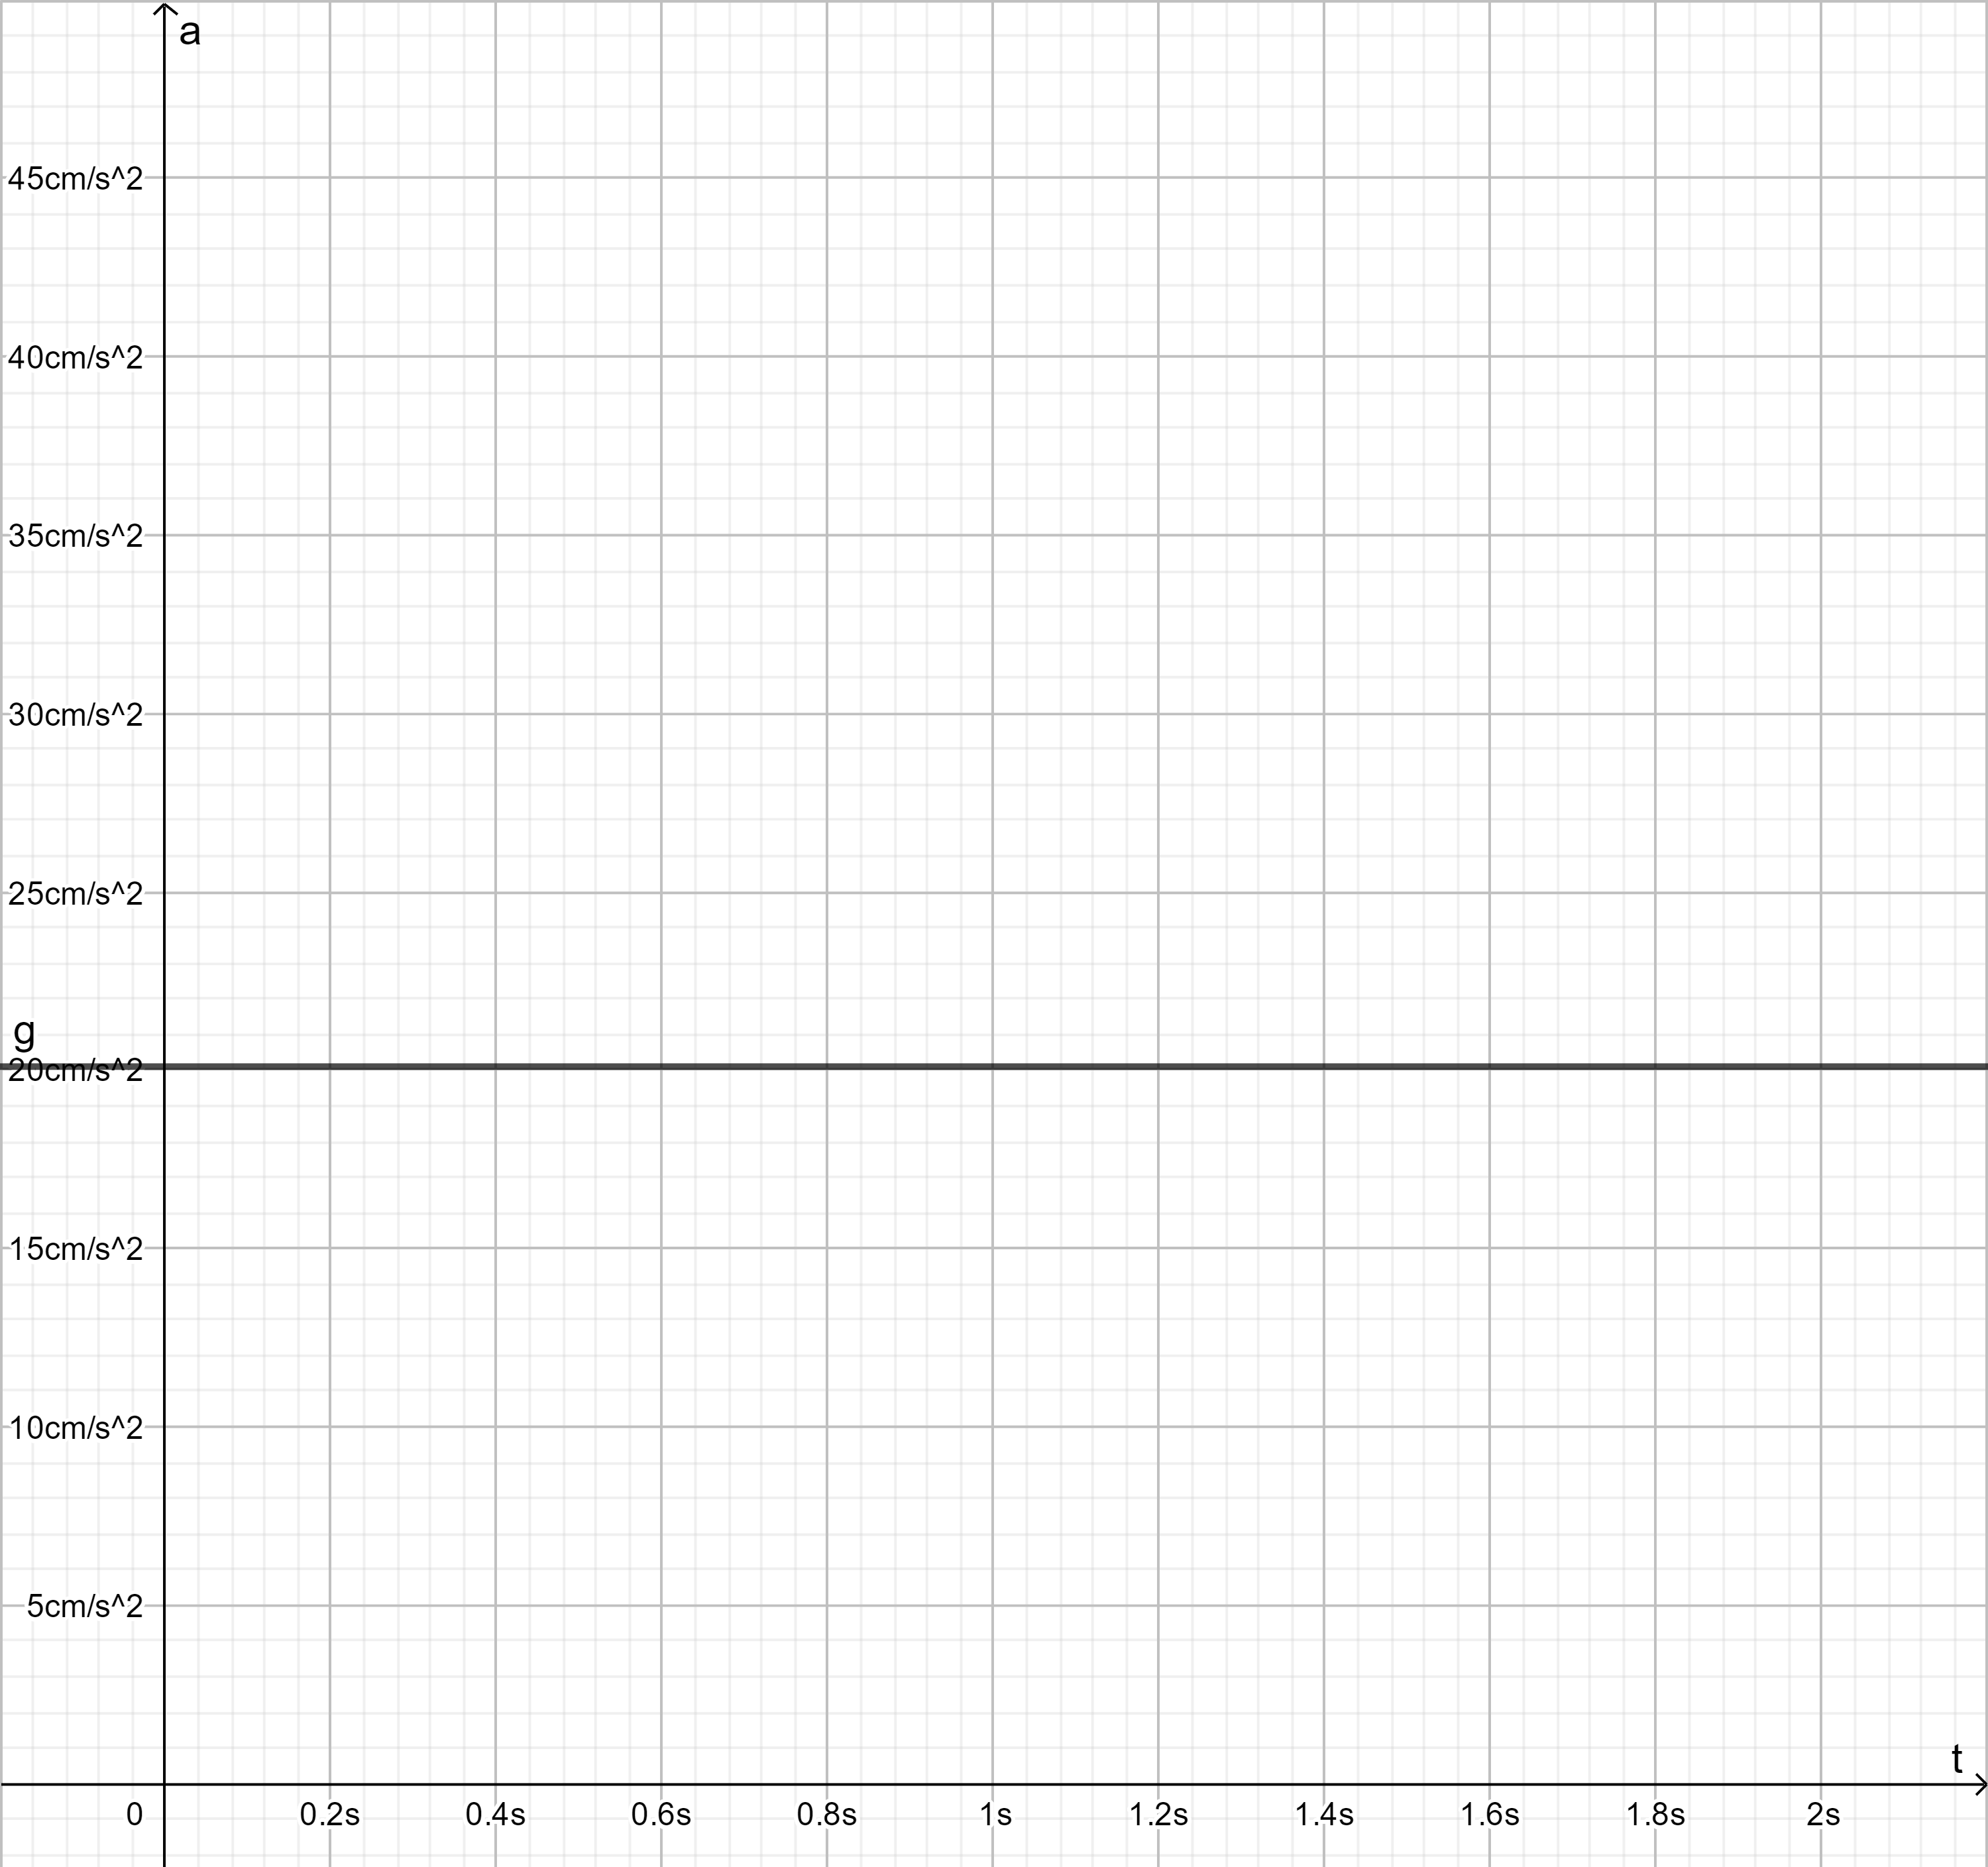
\includegraphics[scale=1.25]{LabReportImg/3TB-Acceleration.png}
            \captionof*{figure}{Trial two: $\vec{a}=0.201$}
        \end{minipage}
    \end{figure}
    \item The acceleration down the ramp ($\vec{a}$) is defined by the formula $\vec{a}=\vec{g}sin\theta$, therefore $g=\frac{a}{sin\theta}$ where $g$ is the acceleration due to gravity and ($a$) is the acceleration along the ramp.
    \begin{itemize}
        \item Trial One:
        \begin{align*}
            g&=\frac{a}{sin\theta}\\
             &=\frac{0.391}{sin(2.99^{\circ})}\\
             &=7.50
        \end{align*}
        \item Trial Two:
        \begin{align*}
            g&=\frac{a}{sin\theta}\\
             &=\frac{0.201}{sin(1.79^{\circ})}\\
             &=6.43
        \end{align*}
    \end{itemize}
    \item Compare the experimental value of $g$ to the theoretical value of $g=$\SI{9.81}{\metre\per\second\squared} using the percentage of error calculation and the percentage of difference for the two values you got.
    \begin{itemize}
        \item Trial One:
        \begin{multicols}{2}
            \begin{align*}
                \% of Error &= \frac{|Approx - Exact|}{|Exact|}\\
                &=\frac{|7.5-9.81|}{9.81}\\
                &=23.5\%
            \end{align*}\break
            \begin{align*}
                \% of Difference &= |\frac{Approx - Exact}{\frac{Approx+Exact}{2}}|\\
                &=|\frac{7.5-9.81}{\frac{7.5+9.81}{2}}|\\
                &=26.7\%
            \end{align*}
        \end{multicols}
        \item Trial Two:
        \begin{multicols}{2}
            \begin{align*}
                \% of Error &= \frac{|Approx - Exact|}{|Exact|}\\
                &=\frac{|6.43-9.81|}{9.81}\\
                &=34.5\%
            \end{align*}\break
            \begin{align*}
                \% of Difference &= |\frac{Approx - Exact}{\frac{Approx+Exact}{2}}|\\
                &=|\frac{6.43-9.81}{\frac{6.43+9.81}{2}}|\\
                &=41.6\%
            \end{align*}
        \end{multicols}
    \end{itemize}
    \item Compare the experimental graphical value of $g$ to the theoretical value of $g=$\SI{9.81}{\metre\per\second\squared} using the percentage of error calculation and the percentage of difference for the two values you got.
    \begin{itemize}
        \item Trial One:
        \begin{multicols}{2}
            \begin{align*}
                \% of Error &= \frac{|Approx - Exact|}{|Exact|}\\
                &=\frac{|7.5-9.81|}{9.81}\\
                &=23.5\%
            \end{align*}\break
            \begin{align*}
                \% of Difference &= |\frac{Approx - Exact}{\frac{Approx+Exact}{2}}|\\
                &=|\frac{7.5-9.81}{\frac{7.5+9.81}{2}}|\\
                &=26.7\%
            \end{align*}
        \end{multicols}
        \item Trial Two:
        \begin{multicols}{2}
            \begin{align*}
                \% of Error &= \frac{|Approx - Exact|}{|Exact|}\\
                &=\frac{|6.43-9.81|}{9.81}\\
                &=34.5\%
            \end{align*}\break
            \begin{align*}
                \% of Difference &= |\frac{Approx - Exact}{\frac{Approx+Exact}{2}}|\\
                &=|\frac{6.43-9.81}{\frac{6.43+9.81}{2}}|\\
                &=41.6\%
            \end{align*}
        \end{multicols}
    \end{itemize}
\end{enumerate}
\begin{enumerate}
    \item Determine an equation for the position time graph. The graph is a parabola and its vertex is the origin (0,0), therefore the equation is $\Delta\vec{d}=k\Delta\vec{t}^2$. Where $\Delta d$ is the displacement in (m), $\Delta t$ is the time in (s), and k is a constant.
    \item Determine the value of the constant k for from the coordinate of three points that you drew tangents at them before in the graphical method. Be sure to determine and include the units for k.
    \begin{center}
        \begin{tabular}{c|c|c @{\hspace{5em}} c|c|c}
            \multicolumn{3}{c}{Trial 1}&\multicolumn{3}{c}{Trial 2}\\
            \hline
            $\Delta t$&$\Delta \vec{d}$&$\frac{\Delta\vec{d}}{\Delta t^2}=k$&$\Delta t$&$\Delta \vec{d}$&$\frac{\Delta\vec{d}}{\Delta t^2}=k$\\
            0.6&0.089&0.247&0.6&0.059&0.164\\
            1.2&0.318&0.221&1.2&0.184&0.128\\
            1.8&0.676&0.209&1.8&0.343&0.106\\
        \end{tabular}
    \end{center}
    \item If you have different values for k in the same graph, use the average.
    \begin{itemize}
        \item Trial One:
            \begin{align*}
                k&=\frac{0.247+0.221+0.209}{3}\\
                &=0.226
            \end{align*}
        \item Trial Two:
            \begin{align*}
                k&=\frac{0.164+0.128+0.106}{3}\\
                &=0.133
            \end{align*}
    \end{itemize}
    \item If the cart has a constant acceleration, it motion should follow the equation $\Delta\vec{d}=\frac{1}{2}\vec{a}\Delta t^2$. The initial velocity of the cart is zero so the equation becomes $\Delta\vec{d}=\vec{v_1}\Delta t+\frac{1}{2}\vec{a}\Delta t^2$. It looks similar to the equation you derived using mathematical modelling therefore $k=\frac{1}{2}a$, where a is the acceleration along the ramp.
    \begin{itemize}
        \item Trial One:
        \begin{align*}
            a=2k\\
           & =2*0.226\\
            &=0.452
        \end{align*}
        \item Trial Two:
        \begin{align*}
            a=2k\\
            &=2*0.133\\
            &=0.266
        \end{align*}
    \end{itemize}
    \item Theoretically $a=g\sin\theta$, where ($\theta$) is the angle of inclination of the ramp and (g) is the acceleration due to gravity. Therefore $k=\frac{1}{2}g\sin\theta$ and $g=\frac{2k}{\sin\theta}$.
    \begin{itemize}
        \item Trial One:
        \begin{align*}
            g&=\frac{a}{sin\theta}\\
             &=\frac{0.452}{sin(2.99^{\circ})}\\
             &=8.67
        \end{align*}
        \item Trial Two:
        \begin{align*}
            g&=\frac{a}{sin\theta}\\
             &=\frac{0.226}{sin(1.79^{\circ})}\\
             &=7.24
        \end{align*}
    \end{itemize}
    \item Compare the experimental value of g to the theoretical value of $g=$\SI{9.81}{\metre\per\second\squared} using the percentage of error calculation and the percentage of difference for the two values you got.
    \begin{itemize}
        \item Trial One:
        \begin{multicols}{2}
            \begin{align*}
                \% of Error &= \frac{|Approx - Exact|}{|Exact|}\\
                &=\frac{|8.76-9.81|}{9.81}\\
                &=10.7\%
            \end{align*}\break
            \begin{align*}
                \% of Difference &= |\frac{Approx - Exact}{\frac{Approx+Exact}{2}}|\\
                &=|\frac{8.76-9.81}{\frac{8.76+9.81}{2}}|\\
                &=11.3\%
            \end{align*}
        \end{multicols}
        \item Trial Two:
        \begin{multicols}{2}
            \begin{align*}
                \% of Error &= \frac{|Approx - Exact|}{|Exact|}\\
                &=\frac{|7.24-9.81|}{9.81}\\
                &=26.2\%
            \end{align*}\break
            \begin{align*}
                \% of Difference &= |\frac{Approx - Exact}{\frac{Approx+Exact}{2}}|\\
                &=|\frac{7.24-9.81}{\frac{7.24+9.81}{2}}|\\
                &=30.1\%
            \end{align*}
        \end{multicols}
    \end{itemize}
\end{enumerate}
\section{Conclusion}
Did the cart experience uniform motion, uniform acceleration or non-uniform acceleration while moving down the ramp? Explain how you know it experienced this type of motion. Use your velocity-time graph to justify graph to justify your explanation.

The cart experienced uniform acceleration. If the object is uniform acceleration, it's acceleration-time graph would be a horizontal line, while it's velocity-time graph would be a linear line. Looking at the velocity-time graph for both trials, we see that they are linear. I also know this cart experienced uniform acceleration as the position-time graph shows a parabolic shape.
\newpage
\section{Source of Error}
State all the human and equipment sources of error, within the lab, that may have affected your results.

\begin{itemize}
    \item Lubrication of the cart
    \item Debris along the track
    \item Friction along the track
    \item Rough measurements of textbooks
    \item Miscounting the dots
\end{itemize}
\end{document}